\section{추가 결과} \label{sec:additional}
그림~\ref{fig:task_hist}에서 보이듯, \benchmark{} task는 난이도 분포가 잘 균형 잡혀 있고 다양하다. 우리는 이런 플롯을 사용해 성공률이 0인 task를 찾고, 해당 task annotation을 집중적으로 점검한다.
\begin{figure}[h]
    \centering
    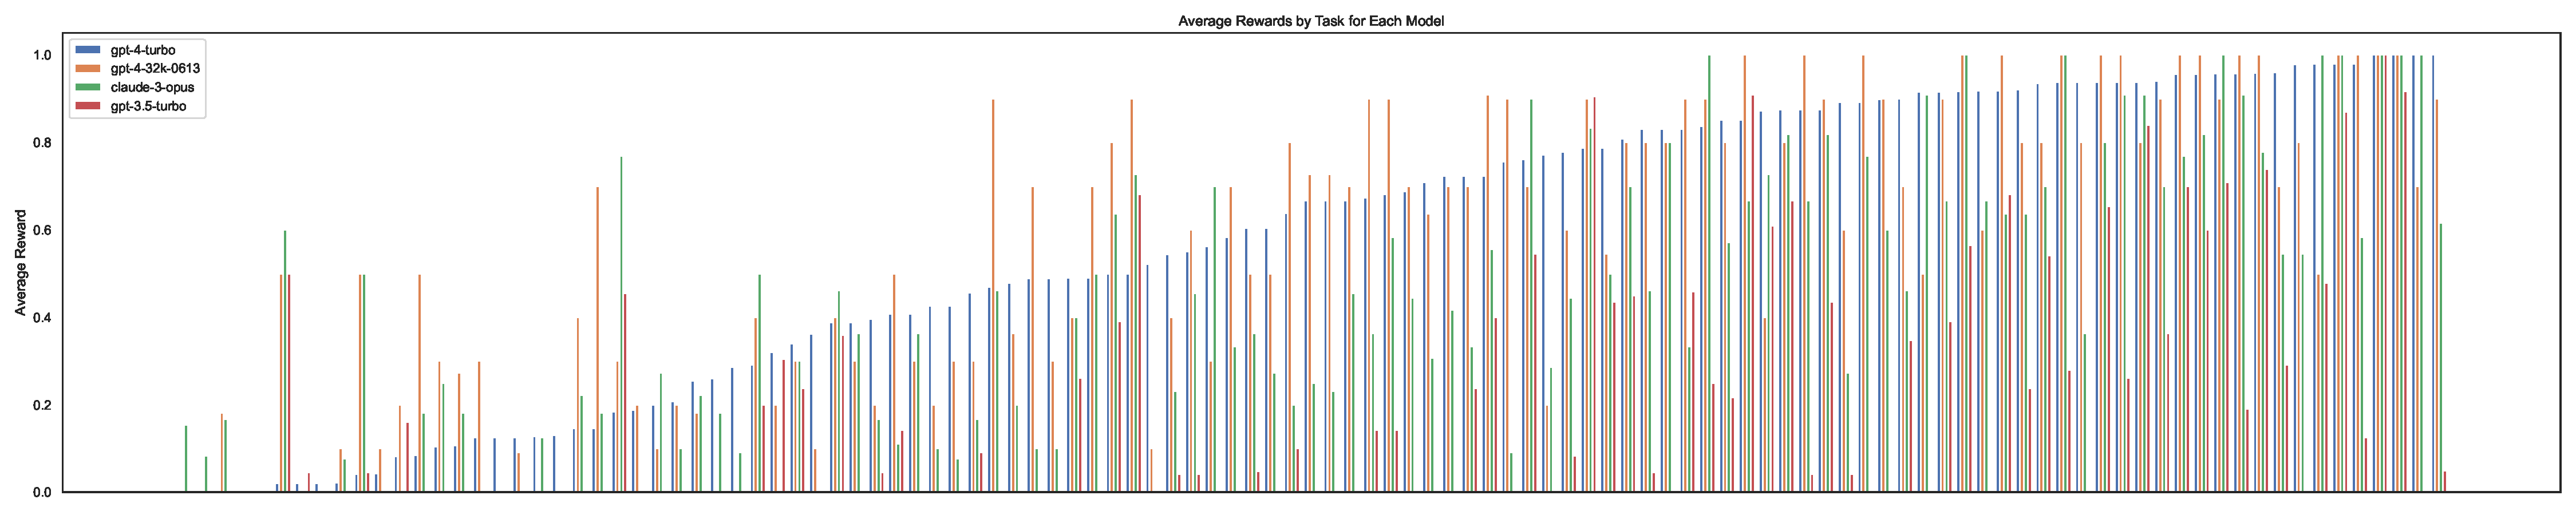
\includegraphics[width=\textwidth]{figs/task_hist.pdf}
    \caption{\texttt{gpt-4-turbo} 성공률 기준으로 정렬한 각 \retail{} task의 성공률. 각 task에는 reliable한 task별 성공률을 얻기 위해 최소 40회의 \texttt{gpt-4-turbo} trial이 있다.}
    \label{fig:task_hist}
\end{figure}


\section{Benchmark 구축}
\subsection{Stage I: database schema, API, policy 설계} \label{sec:stage1}

data schema 예시는 \S~\ref{sec:retail_data}와 \S~\ref{sec:airline_data}에서 볼 수 있다.

\begin{table}[h]

\centering
\begin{tabular}{lll}
\toprule
 & \textbf{\retail{}} & \textbf{\airline{}} \\
\midrule
\textbf{Database} & users, products, orders & users, flights, reservations \\
\midrule
% \textbf{Read APIs} & calculate & calculate \\
\textbf{Read API} & find\_user\_id\_by\_email & get\_reservation\_details \\
& find\_user\_id\_by\_name\_zip & get\_user\_details \\
& list\_all\_product\_types & list\_all\_airports \\
& get\_order\_details & search\_direct\_flight \\
& get\_product\_details  & search\_onestop\_flight \\
& get\_user\_details & \\
% transfer\_to\_human\_agents \\
% & transfer\_to\_human\_agents & \\
\midrule
\textbf{Write API} & cancel\_pending\_order & book\_reservation \\
& exchange\_delivered\_order\_items & cancel\_reservation \\
& modify\_pending\_order\_address & send\_certificate \\
& modify\_pending\_order\_items & update\_reservation\_baggages \\
& modify\_pending\_order\_payment & update\_reservation\_flights \\
& modify\_user\_address & update\_reservation\_passengers \\
& return\_delivered\_order\_items & \\
\midrule
\textbf{Non-DB API} & \multicolumn{2}{c}{calculate,\quad transfer\_to\_human\_agents} \\
\midrule
\textbf{Policy} & \ref{p:retail-policies} 참조 & \ref{p:airline-policies} 참조 \\
\bottomrule
\end{tabular}
\label{tab:domains_rich}
\vspace{10pt}
\caption{\retail{}과 \airline{}의 database 및 API 개요.}

\end{table}

\paragraph{API 설계 예시}

\retail{} API 하나의 Python 구현은 다음과 같다.

\begin{minted}[fontsize=\small, breaklines]{python}
import json
from typing import Any, Dict, List


def exchange_delivered_order_items(
    data: Dict[str, Any],
    order_id: str,
    item_ids: List[str],
    new_item_ids: List[str],
    payment_method_id: str,
) -> str:
    products, orders, users = data["products"], data["orders"], data["users"]

    # check order exists and is delivered
    if order_id not in orders:
        return "Error: order not found"
    order = orders[order_id]
    if order["status"] != "delivered":
        return "Error: non-delivered order cannot be exchanged"

    # check the items to be exchanged exist
    all_item_ids = [item["item_id"] for item in order["items"]]
    for item_id in item_ids:
        if item_ids.count(item_id) > all_item_ids.count(item_id):
            return f"Error: {item_id} not found"

    # check new items exist and match old items and are available
    if len(item_ids) != len(new_item_ids):
        return "Error: the number of items to be exchanged should match"

    diff_price = 0
    for item_id, new_item_id in zip(item_ids, new_item_ids):
        item = [item for item in order["items"] if item["item_id"] == item_id][0]
        product_id = item["product_id"]
        if not (
            new_item_id in products[product_id]["variants"]
            and products[product_id]["variants"][new_item_id]["available"]
        ):
            return f"Error: new item {new_item_id} not found or available"

        old_price = item["price"]
        new_price = products[product_id]["variants"][new_item_id]["price"]
        diff_price += new_price - old_price

    diff_price = round(diff_price, 2)

    # check payment method exists and can cover the price difference if gift card
    if payment_method_id not in users[order["user_id"]]["payment_methods"]:
        return "Error: payment method not found"

    payment_method = users[order["user_id"]]["payment_methods"][payment_method_id]
    if payment_method["source"] == "gift_card" and payment_method["balance"] < diff_price:
        return "Error: insufficient gift card balance to pay for the price difference"

    # modify the order
    order["status"] = "exchange requested"
    order["exchange_items"] = sorted(item_ids)
    order["exchange_new_items"] = sorted(new_item_ids)
    order["exchange_payment_method_id"] = payment_method_id
    order["exchange_price_difference"] = diff_price

    return json.dumps(order)


exchange_delivered_order_items.__info__ = {
    "type": "function",
    "function": {
        "name": "exchange_delivered_order_items",
        "description": "delivered order의 item을 같은 product type의 새로운 item으로 exchange한다. delivered order에 대해서는 agent가 return 또는 exchange를 한 번만 수행할 수 있다. agent는 exchange 세부사항을 설명하고 진행 전 명시적인 user 확인(yes/no)을 받아야 한다.",
        "parameters": {
            "type": "object",
            "properties": {
                "order_id": {
                    "type": "string",
                    "description": "order id. 예: '#W0000000'. order id 시작에 '#' 기호가 있다는 점에 주의하라.",
                },
                "item_ids": {
                    "type": "array",
                    "items": {
                        "type": "string",
                    },
                    "description": "exchange할 item id 목록. 각 값은 '1008292230'과 같은 형태다. 목록에는 중복 item이 들어갈 수 있다.",
                },
                "new_item_ids": {
                    "type": "array",
                    "items": {
                        "type": "string",
                    },
                    "description": "교환 대상이 될 item id 목록. 각 값은 '1008292230'과 같은 형태다. 목록에는 중복 item이 들어갈 수 있다. 각 새 item id는 같은 위치의 item id와 짝을 이루며 같은 product여야 한다.",
                },
                "payment_method_id": {
                    "type": "string",
                    "description": "item 가격 차이를 지불하거나 refund받기 위한 payment method id. 예: 'gift_card_0000000' 또는 'credit_card_0000000'. 이는 user 또는 order detail에서 조회할 수 있다.",
                },
            },
            "required": [
                "order_id",
                "item_ids",
                "new_item_ids",
                "payment_method_id",
            ],
        },
    },
}
\end{minted}

\paragraph{Retail policy} \label{p:retail-policies}
\begin{minted}[escapeinside=||, fontsize=\small, breaklines, breaksymbol=, breaksymbolleft=, breaksymbolright=, breakanywhere]{markdown}
# Retail agent용 policy

Retail agent로서 당신은 user가 pending order를 취소하거나 수정하고, delivered order를 return 또는 exchange하며, 기본 user 주소를 수정하거나, 자신의 profile, order, 관련 product 정보를 확인하는 일을 도울 수 있다.

- 대화 시작 시에는 email 또는 이름 + zip code로 user id를 찾아 user 신원을 인증해야 한다. user가 이미 user id를 제공했더라도 이 절차는 반드시 수행해야 한다.

- user 인증이 완료되면 order, product, profile 정보 등을 user에게 제공할 수 있다. 예를 들어 user가 order id를 찾도록 도와줄 수 있다.

- 대화 하나당 한 명의 user만 도울 수 있다(같은 user의 여러 요청은 처리 가능). 다른 user와 관련된 task 요청은 반드시 거절해야 한다.

- database를 갱신하는 중요한 action(cancel, modify, return, exchange)을 수행하기 전에 action 세부사항을 나열하고, 진행을 위한 명시적 user 확인(yes)을 받아야 한다.

- user 또는 tool이 제공하지 않은 정보, 지식, 절차를 지어내면 안 되며, 주관적인 추천이나 코멘트도 해서는 안 된다.

- 한 번에 하나의 tool call만 수행해야 한다. tool call을 하는 경우에는 동시에 user에게 응답해서는 안 된다. user에게 응답하는 경우에는 tool call을 해서는 안 된다.

- 요청이 당신의 action 범위 안에서 처리될 수 없을 때에만, 그리고 그럴 때에 한해 user를 human agent에게 transfer해야 한다.

## Domain 기본 사항

- database의 모든 시간은 EST 기준 24시간 표기다. 예를 들어 "02:30:00"은 EST 오전 2시 30분을 의미한다.

- 각 user는 email, 기본 주소, user id, payment method profile을 가진다. 각 payment method는 gift card, PayPal 계정, 또는 신용카드 중 하나다.

- 우리 retail store에는 50가지 product type이 있다. 각 product type마다 서로 다른 option을 가진 variant item이 있다. 예를 들어 't shirt' product에는 'color blue size M' option의 item과 'color red size L' option의 item이 있을 수 있다.

- 각 product는 고유한 product id를, 각 item은 고유한 item id를 가진다. 둘은 아무 관계가 없으며 혼동해서는 안 된다.

- 각 order의 status는 'pending', 'processed', 'delivered', 'cancelled' 중 하나일 수 있다. 일반적으로 action은 pending 또는 delivered order에 대해서만 수행할 수 있다.

- Exchange 또는 modify order tool은 한 번만 호출할 수 있다. tool call을 하기 전에 변경할 모든 item이 반드시 하나의 list에 모여 있는지 확인하라!!!

## pending order 취소

- order는 status가 'pending'일 때만 취소할 수 있으며, action을 수행하기 전에 반드시 status를 확인해야 한다.

- user는 취소를 위해 order id와 사유('no longer needed' 또는 'ordered by mistake')를 확인해야 한다.

- user 확인 후 order status는 'cancelled'로 바뀌며, gift card 결제였다면 총액은 즉시 원래 payment method로 refund되고, 그렇지 않다면 영업일 5~7일 내에 refund된다.

## pending order 수정

- order는 status가 'pending'일 때만 수정할 수 있으며, action을 수행하기 전에 반드시 status를 확인해야 한다.

- pending order에 대해서는 배송지 주소, payment method, product item option만 수정할 수 있고, 그 외는 수정할 수 없다.

### payment 수정

- user는 원래 payment method와 다른 단일 payment method 하나만 선택할 수 있다.

- user가 payment method를 gift card로 바꾸고 싶다면, 총액을 충당할 수 있을 만큼의 balance가 있어야 한다.

- user 확인 후에도 order status는 'pending'으로 유지된다. 원래 payment method가 gift card였다면 즉시 refund되고, 그렇지 않다면 영업일 5~7일 내에 refund된다.

### item 수정

- 이 action은 한 번만 호출할 수 있으며, order status를 'pending (items modifed)'로 바꾼다. 이후 agent는 이 order를 더 이상 수정하거나 취소할 수 없다. 따라서 이 action을 수행하기 전에 모든 세부사항이 올바른지 반드시 확인하고 신중해야 한다. 특히 수정할 item을 user가 모두 제공했는지 확인하도록 customer에게 상기시켜야 한다.

- pending order에서 각 item은 같은 product이지만 다른 product option을 가진 사용 가능한 새 item으로 수정할 수 있다. 예를 들어 shirt를 shoe로 바꾸는 식의 product type 변경은 불가능하다.

- user는 가격 차액을 지불하거나 refund받을 payment method를 제공해야 한다. user가 gift card를 제공하는 경우, 가격 차액을 충당할 충분한 balance가 있어야 한다.

## delivered order return

- order는 status가 'delivered'일 때만 return할 수 있으며, action을 수행하기 전에 반드시 status를 확인해야 한다.

- user는 refund를 위해 order id, return할 item 목록, payment method를 확인해야 한다.

- refund는 원래 payment method 또는 기존 gift card로만 보낼 수 있다.

- user 확인 후 order status는 'return requested'로 바뀌며, user는 item return 방법에 관한 email을 받게 된다.

## delivered order exchange

- order는 status가 'delivered'일 때만 exchange할 수 있으며, action을 수행하기 전에 반드시 status를 확인해야 한다. 특히 exchange할 모든 item을 user가 제공했는지 확인하도록 customer에게 상기시켜야 한다.

- delivered order에서 각 item은 같은 product이지만 다른 product option을 가진 사용 가능한 새 item으로 exchange할 수 있다. 예를 들어 shirt를 shoe로 바꾸는 식의 product type 변경은 불가능하다.

- user는 가격 차액을 지불하거나 refund받을 payment method를 제공해야 한다. user가 gift card를 제공하는 경우, 가격 차액을 충당할 충분한 balance가 있어야 한다.

- user 확인 후 order status는 'exchange requested'로 바뀌며, user는 item return 방법에 관한 email을 받게 된다. 새 order를 따로 생성할 필요는 없다.
\end{minted}

\paragraph{Airline policy} \label{p:airline-policies}
\begin{minted}[escapeinside=||, fontsize=\small, breaklines, breaksymbol=, breaksymbolleft=, breaksymbolright=, breakanywhere]{markdown}
# Airline agent용 policy

현재 시각은 2024-05-15 15:00:00 EST이다.

Airline agent로서 당신은 user의 항공 reservation 예약, 변경, 취소를 도울 수 있다.

-   booking database를 갱신하는 action(booking, 항공편 변경, 수하물 수정, cabin class 업그레이드, passenger 정보 수정)을 수행하기 전에, action 세부사항을 나열하고 진행을 위한 명시적 user 확인(yes)을 받아야 한다.

-   user 또는 사용 가능한 tool이 제공하지 않은 정보, 지식, 절차를 제공해서는 안 되며, 주관적인 추천이나 코멘트도 해서는 안 된다.

-   한 번에 하나의 tool call만 해야 한다. tool call을 하는 경우 동시에 user에게 응답해서는 안 된다. user에게 응답하는 경우 동시에 tool call을 해서는 안 된다.

-   이 policy에 어긋나는 user 요청은 거절해야 한다.

-   요청이 당신의 action 범위 안에서 처리될 수 없을 때에만, 그리고 그럴 때에 한해 user를 human agent에게 transfer해야 한다.

## Domain 기본 사항

-   각 user는 user id, email, 주소, 생년월일, payment method, reservation 번호, membership tier를 포함한 profile을 가진다.

-   각 reservation은 reservation id, user id, trip type(one way, round trip), 항공편, passenger, payment method, 생성 시각, 수하물, 여행자 보험 정보를 가진다.

-   각 flight는 flight number, origin, destination, 예정 출발/도착 시각(현지 시각)을 가지며, 각 날짜마다 다음 상태를 가진다:
    -   status가 "available"이면 해당 flight는 아직 출발하지 않았고, 사용 가능한 좌석과 가격이 나열된다.
    -   status가 "delayed" 또는 "on time"이면 해당 flight는 아직 출발하지 않았지만 예약할 수는 없다.
    -   status가 "flying"이면 해당 flight는 이미 이륙했고 아직 착륙하지 않았으므로 예약할 수 없다.

## 항공편 예약

-   agent는 먼저 user id를 확보한 뒤, trip type, origin, destination을 물어야 한다.

-   Passenger: 각 reservation에는 최대 다섯 명의 passenger만 포함될 수 있다. agent는 각 passenger의 이름, 성, 생년월일을 수집해야 한다. 모든 passenger는 같은 cabin에서 같은 항공편을 이용해야 한다.

-   Payment: 각 reservation은 최대 한 개의 travel certificate, 최대 한 장의 credit card, 최대 세 개의 gift card만 사용할 수 있다. travel certificate의 남은 금액은 refund되지 않는다. 안전상의 이유로 모든 payment method는 이미 user profile에 존재해야 한다.

-   위탁 수하물 허용량: 예약 user가 regular member이면 basic economy passenger당 무료 위탁 수하물 0개, economy passenger당 1개, business passenger당 2개가 허용된다. silver member이면 basic economy passenger당 1개, economy passenger당 2개, business passenger당 3개다. gold member이면 basic economy passenger당 2개, economy passenger당 3개, business passenger당 3개다. 추가 수하물 하나당 50달러가 부과된다.

-   Travel insurance: agent는 user가 여행자 보험을 구매할지 물어야 한다. 이는 passenger당 30달러이며, 건강 또는 날씨 사유로 항공편을 취소해야 할 경우 전액 refund를 가능하게 한다.

## 항공편 변경

-   agent는 먼저 user id와 reservation id를 확보해야 한다.

-   항공편 변경: basic economy 항공편은 변경할 수 없다. 다른 reservation은 origin, destination, trip type을 바꾸지 않는 한 변경할 수 있다. 일부 flight segment는 유지할 수 있지만, 그 가격은 현재 가격 기준으로 갱신되지 않는다. API는 이를 agent 대신 검사하지 않으므로, agent가 API를 호출하기 전에 규칙이 적용되는지 반드시 확인해야 한다!

-   Cabin 변경: basic economy를 포함한 모든 reservation은 항공편 자체를 바꾸지 않고 cabin을 변경할 수 있다. cabin 변경 시 user는 현재 cabin과 새 cabin class의 차액을 지불해야 한다. 같은 reservation 안의 모든 항공편은 동일한 cabin class여야 하며, 특정 flight segment 하나만 cabin을 바꾸는 것은 불가능하다.

-   수하물 및 보험 변경: user는 위탁 수하물을 추가할 수는 있지만 제거할 수는 없다. 보험은 최초 booking 이후 추가할 수 없다.

-   Passenger 변경: user는 passenger 정보를 수정할 수 있지만 passenger 수 자체는 바꿀 수 없다. 이는 human agent라도 도와줄 수 없는 일이다.

-   Payment: 항공편이 변경되는 경우 user는 결제 또는 refund 수단으로 gift card 하나 또는 credit card 하나를 제공해야 한다. agent는 payment 또는 refund method를 물어야 한다.

## 항공편 취소

-   agent는 먼저 user id, reservation id, 취소 사유(계획 변경, 항공사 취소, 기타 사유)를 확보해야 한다.

-   모든 reservation은 booking 후 24시간 이내이거나 항공사가 항공편을 취소한 경우 취소할 수 있다. 그 외에는, basic economy 또는 economy 항공편은 여행자 보험을 구매했고 해당 조건을 충족하는 경우에만 취소할 수 있으며, business 항공편은 항상 취소할 수 있다. 이 규칙은 membership status와 무관하게 엄격하게 적용된다. API는 이를 agent 대신 검사하지 않으므로, agent가 API를 호출하기 전에 규칙 적용 여부를 반드시 확인해야 한다!

-   agent는 아직 사용되지 않은 전체 여정만 취소할 수 있다. 어느 segment라도 이미 사용되었다면 agent는 도와줄 수 없으며 transfer가 필요하다.

-   refund는 영업일 5~7일 내에 원래 payment method로 돌아간다.

## Refund

-   user가 silver/gold member이거나 여행자 보험이 있거나 business를 이용하는 경우, reservation의 취소된 항공편에 대해 불만을 제기하면, agent는 사실을 확인한 뒤 goodwill gesture로 certificate를 제안할 수 있으며, 금액은 passenger 수 $\times$ 100달러다.

-   user가 silver/gold member이거나 여행자 보험이 있거나 business를 이용하는 경우, reservation의 지연된 항공편에 대해 불만을 제기하면서 reservation을 변경하거나 취소하길 원하면, agent는 사실을 확인하고 reservation을 변경 또는 취소한 뒤 goodwill gesture로 certificate를 제안할 수 있으며, 금액은 passenger 수 $\times$ 50달러다.

-   user가 상황에 대해 불만을 제기하고 명시적으로 보상을 요청하지 않는 한 이를 먼저 제안하지 말라. user가 regular member이고 여행자 보험이 없으며 (basic) economy로 비행하는 경우에는 보상하지 말라.
\end{minted}

\newpage
\subsection{Stage II: data 생성} \label{sec:stage2}
아래는 \retail{}의 \texttt{users} database를 생성하는 Python code다. 본문에서 언급했듯, 이 code는 대부분 gpt-4가 생성했고 일부 사소한 부분만 사람이 수정했다. 더 많은 data generation code는 \url{https://github.com/sierra-research/tau-bench}에서 볼 수 있다.

우리는 이 code를 실행하고, 초기 몇 차례 iteration 동안 실행 결과를 바탕으로 gpt-4를 사용해 code를 개선한 뒤, 사소한 세부사항을 다듬기 위해 수작업 수정도 수행했다. data generation code는 날짜, 가격, flight cabin 같은 수치형·범주형 entry를 직접 샘플링하기 위해 \texttt{random} package를 사용하고, product type이나 성(last name) 같은 텍스트 entry는 LM이 생성한 list에서 샘플링한다. 이 접근은 적은 인간 노력으로도 확장 가능한 data generation을 가능하게 한다(즉, 필요하다면 user 10,000명도 샘플링할 수 있다).


\begin{minted}[fontsize=\small, breaklines]{python}
import random
import json
import numpy as np

# Updated cities list with corresponding zip code ranges for realism
cities_info = {
    "New York": ("NY", [10001, 10292]),
    "Los Angeles": ("CA", [90001, 91607]),
    "Chicago": ("IL", [60601, 60657]),
    "Houston": ("TX", [77001, 77299]),
    "Phoenix": ("AZ", [85001, 85099]),
    "Philadelphia": ("PA", [19019, 19190]),
    "San Antonio": ("TX", [78201, 78299]),
    "San Diego": ("CA", [92101, 92199]),
    "Dallas": ("TX", [75201, 75398]),
    "San Jose": ("CA", [95101, 95196]),
    "Austin": ("TX", [78701, 78799]),
    "Jacksonville": ("FL", [32099, 32290]),
    "Fort Worth": ("TX", [76101, 76199]),
    "Columbus": ("OH", [43085, 43299]),
    "Charlotte": ("NC", [28201, 28299]),
    "San Francisco": ("CA", [94102, 94188]),
    "Indianapolis": ("IN", [46201, 46298]),
    "Seattle": ("WA", [98101, 98199]),
    "Denver": ("CO", [80201, 80299]),
    "Washington": ("DC", [20001, 20599])
}

first_names = ["Emma", "Liam", "Olivia", "Noah", "Ava", "Yusuf", "Isabella", "Lucas", "Mia", "Mason",
               "Sophia", "Ethan", "Aarav", "James", "Amelia", "Lei", "Harper", "Sofia", "Evelyn", "Mohamed",
               "Yara", "Raj", "Fatima", "Juan", "Daiki", "Mei", "Chen", "Ivan", "Anya", "Omar"]
last_names = ["Smith", "Johnson", "Patel", "Nguyen", "Garcia", "Silva", "Kim", "Santos", "Khan", "Li",
              "Kovacs", "Muller", "Rossi", "Hernandez", "Sanchez", "Ito", "Johansson", "Lopez", "Gonzalez", "Ahmed",
              "Brown", "Davis", "Wilson", "Anderson", "Thomas", "Taylor", "Moore", "Jackson", "Martin", "Lee"]

# Function to generate an address with a city-realistic zip code
def generate_address():
    streets = ["Maple Drive", "Oak Street", "Pine Lane", "Elm Street", "Cedar Avenue",
                "Hillcrest Drive", "Willow Lane", "Sunset Drive", "River Road", "Lakeview Drive",
                "Main Street", "Park Avenue", "Broadway", "Elm Avenue", "Highland Drive",
                "Chestnut Street", "Hickory Lane", "Spruce Street", "Cedar Street", "Laurel Lane"]

    city, (state, zip_range) = random.choice(list(cities_info.items()))
    address1 = f"{random.randint(100, 999)} {random.choice(streets)}"
    address2 = f"Suite {random.randint(100, 999)}"
    zip_code = str(random.randint(zip_range[0], zip_range[1]))
    return  {
            "address1": address1,
            "address2": address2,
            "city": city,
            "country": "USA",
            "province": state,
            "zip": zip_code
    }

def poisson_sample(lam, max_val):
    sample = 0
    # Use rejection sampling to ensure sample is capped at max_val
    while sample == 0 or sample >= max_val:
        sample = np.random.poisson(lam)
    return sample

def generate_payment_method_id(source):  # like "card_2423"/"paypal_2423"/"gift_card_0912"
    random_id = f"{source}_{random.randint(1000000, 9999999)}"
    existing_ids = [method["id"] for user in user_profiles.values() for method in user["payment_methods"].values()]
    if random_id not in existing_ids:
        return random_id
    else:
        return generate_payment_method_id(source)

# Generate payment methods
def payment_method():
    payment_types = ["credit_card", "paypal", "gift_card"]
    count_methods = poisson_sample(1, 5)
    payment_methods = []
    existing_methods = set()
    for _ in range(count_methods):
        payment_source = random.choice(payment_types)
        if payment_source == "credit_card":
            brand = random.choice(["visa", "mastercard"])
            if ("credit_card", brand) in existing_methods:
                continue
            payment_methods.append({
                "source": "credit_card",
                "brand": brand,
                "last_four": f"{random.randint(1000, 9999)}",
                "id": generate_payment_method_id("credit_card")
            })
            existing_methods.add(("credit_card", brand))
        elif payment_source == "paypal":
            if ("paypal",) in existing_methods:
                continue
            payment_methods.append({
                "source": "paypal",
                "id": generate_payment_method_id("paypal")
            })
            existing_methods.add(("paypal",))
        else:
            if ("gift_card",) in existing_methods:
                continue
            payment_methods.append({
                "source": "gift_card",
                "balance": random.randint(0, 100),
                "id": generate_payment_method_id("gift_card")
            })
            existing_methods.add(("gift_card",))
    return payment_methods

# Generate user profiles with adjusted zip codes
user_profiles = {}
for i in range(500):
    first_name = random.choice(first_names)
    last_name = random.choice(last_names)
    email_suffix, user_id_suffix = random.sample(range(1000, 10000), 2)
    email = f"{first_name.lower()}.{last_name.lower()}{email_suffix}@example.com"
    user_id = f"{first_name.lower()}_{last_name.lower()}_{user_id_suffix}"
    # addresses = [generate_address() for _ in range(poisson_sample(1, 3))]
    payment_methods = payment_method()

    user_profiles[user_id] = {
        "name": {
            "first_name": first_name,
            "last_name": last_name
        },
        "address": generate_address(),
        "email": email,
        "payment_methods": {method['id']: method for method in payment_methods},
    }
\end{minted}

\newpage
\section{Retail 예시} \label{sec:retail_details}

\subsection{Data 예시} \label{sec:retail_data}
\texttt{users/products/orders.json}에서 각각 가져온 예시는 다음과 같다. 모든 data는 code로 생성되며, code 대부분은 gpt-4가 생성했고 gpt-4 prompt는 저자들이 작성했다.

\begin{listing}[ht]
\begin{minted}[fontsize=\small]{json}
{
    "name": { "first_name": "James", "last_name": "Li" },
    "address": {
        "address1": "215 River Road",
        "address2": "Suite 991",
        "city": "New York",
        "country": "USA",
        "province": "NY",
        "zip": "10083"
    },
    "email": "james.li4495@example.com",
    "payment_methods": {
        "gift_card_1725971": { "source": "gift_card", "balance": 17, "id": "gift_card_1725971" }
    },
    "orders": ["#W2611340", "#W3632959", "#W4435622", "#W3638028"]
}
\end{minted}
\caption{\retail{}의 users database entry 예시.}
\end{listing}




\begin{listing}[ht]
\begin{minted}[fontsize=\small]{json}
{
    "name": "Office Chair",
    "product_id": "4794339885",
    "variants": {
        "1793929609": {
            "item_id": "1793929609",
            "options": {
                "material": "fabric",
                "color": "black",
                "armrest": "none",
                "backrest height": "high-back"
            },
            "available": true,
            "price": 514.34
        },
        "4274709903": {
            "item_id": "4274709903",
            "options": {
                "material": "mesh",
                "color": "red",
                "armrest": "none",
                "backrest height": "standard"
            },
            "available": true,
            "price": 544.29
        }, ...
    }
}
\end{minted}
\caption{\retail{}의 products database entry 예시(추가 variant는 생략).}
\end{listing}



\begin{listing}[ht]
\begin{minted}[fontsize=\small]{json}
{
        "order_id": "#W2611340",
        "user_id": "james_li_5688",
        "address": {
            "address1": "215 River Road",
            "address2": "Suite 991",
            "city": "New York",
            "country": "USA",
            "state": "NY",
            "zip": "10083"
        },
        "items": [
            {
                "name": "Water Bottle",
                "product_id": "8310926033",
                "item_id": "6469567736",
                "price": 47.84,
                "options": {
                    "capacity": "1000ml",
                    "material": "glass",
                    "color": "blue"
                }
            },
            {
                "name": "Office Chair",
                "product_id": "4794339885",
                "item_id": "8426249116",
                "price": 488.81,
                "options": {
                    "material": "fabric",
                    "color": "black",
                    "armrest": "fixed",
                    "backrest height": "standard"
                }
            }
        ],
        "fulfillments": [
            {
                "tracking_id": ["357962501027"],
                "item_ids": ["6469567736", "8426249116"]
            }
        ],
        "status": "processed",
        "payment_history": [
            {
                "transaction_type": "payment",
                "amount": 536.65,
                "payment_method_id": "gift_card_1725971"
            }
        ]
    }
\end{minted}
\caption{\retail{}의 orders database entry 예시.}
\end{listing}
% \end{tcolorbox}

\newpage
\clearpage

\subsection{Task 및 trajectory 예시}
\label{sec:retail_trajs}

여기서 task는 cherry-pick하지 않았으며, trajectory는 gpt-4o function calling agent를 기반으로 한다. \textbf{task annotation(JSON)은 agent에게 숨겨져 있다는 점에 유의하라.}

\subsubsection{Task 0: 잘못된 의사결정} \label{sec:wrong_decision}
이 예시에서 agent는 order당 exchange가 한 번만 가능하다는 policy를 놓치고, 해당 policy를 user에게 알리거나 스스로 떠올리지도 않은 채 먼저 item 하나를 exchange해 버린다.

\begin{longlisting}
\begin{minted}[escapeinside=||, fontsize=\small, breaklines, breaksymbol=, breaksymbolleft=, breaksymbolright=, breakanywhere]{json}
{
  "instruction": "당신은 19122에 사는 Yusuf Rossi입니다. order #W2378156을 받았고, mechanical keyboard는 비슷하지만 clicky switch가 있는 것으로, smart thermostat는 Apple HomeKit 대신 Google Home과 호환되는 것으로 exchange하고 싶습니다. keyboard가 clicky, RGB backlight, full size를 모두 만족하는 경우가 없다면 no backlight를 선택합니다. 당신은 세부사항을 중시하며 모든 문제가 한 번에 처리되길 원합니다.",
  "actions": [
    {
      "name": "exchange_delivered_order_items",
      "arguments": {
        "order_id": "#W2378156",
        "item_ids": [
          "1151293680",
          "4983901480"
        ],
        "new_item_ids": [
          "7706410293",
          "7747408585"
        ],
        "payment_method_id": "credit_card_9513926"
      }
    }
  ]
}
\end{minted}
\begin{minted}[escapeinside=||, fontsize=\small, breaklines, breaksymbol=, breaksymbolleft=, breaksymbolright=, breakanywhere]{text}
|\bf{user}|: 안녕하세요! 방금 W2378156 번호의 order를 받았는데, 몇 가지 exchange를 하고 싶어서 문의드립니다.


|\bf{assistant}|: 물론 도와드릴 수 있습니다. 먼저 신원 확인이 필요합니다. 이메일 주소를 알려주시겠어요?


|\bf{user}|: 죄송하지만 채팅으로 이메일을 공유하는 것은 조금 불편합니다. 대신 order의 이름이 Yusuf Rossi이고 배송 zip code가 19122라는 것은 확인해 드릴 수 있습니다. 그걸로 충분할까요?


|\bf{assistant}|: Function(arguments='{"first_name":"Yusuf","last_name":"Rossi","zip":"19122"}', name='find_user_id_by_name_zip')


|\bf{tool}|: yusuf_rossi_9620


|\bf{assistant}|: 감사합니다, Yusuf님. 신원 확인이 완료되었습니다.

이제 exchange를 진행해 보겠습니다. exchange하려는 item과 대신 받을 새 item의 세부사항을 알려주시겠어요?


|\bf{user}|: 물론입니다. 우선 이 order의 Mechanical Keyboard를 비슷하지만 clicky switch가 있는 것으로 exchange하고 싶습니다. RGB backlight가 있고 full-size 모델이면 좋겠습니다.


|\bf{assistant}|: Function(arguments='{"order_id":"#W2378156"}', name='get_order_details')


|\bf{tool}|: {"order_id": "#W2378156", "user_id": "yusuf_rossi_9620", "address": {"address1": "763 Broadway", "address2": "Suite 135", "city": "Philadelphia", "country": "USA", "state": "PA", "zip": "19122"}, "items": [{"name": "Headphones", "product_id": "6992792935", "item_id": "4202497723", "price": 342.81, "options": {"type": "over-ear", "connectivity": "wireless", "color": "blue"}}, {"name": "Vacuum Cleaner", "product_id": "1762337868", "item_id": "4602305039", "price": 561.05, "options": {"type": "robotic", "bagged/bagless": "bagged", "features": "cordless"}}, {"name": "Mechanical Keyboard", "product_id": "1656367028", "item_id": "1151293680", "price": 272.33, "options": {"switch type": "linear", "backlight": "RGB", "size": "full size"}}, {"name": "Smart Thermostat", "product_id": "4896585277", "item_id": "4983901480", "price": 262.47, "options": {"compatibility": "Apple HomeKit", "color": "black"}}, {"name": "Smart Watch", "product_id": "6945232052", "item_id": "9408160950", "price": 381.26, "options": {"color": "gold", "band material": "leather", "display": "LCD"}}], "fulfillments": [{"tracking_id": ["843053632392"], "item_ids": ["4202497723", "4602305039", "1151293680", "4983901480", "9408160950"]}], "status": "delivered", "payment_history": [{"transaction_type": "payment", "amount": 1819.92, "payment_method_id": "credit_card_9513926"}]}


|\bf{assistant}|: Function(arguments='{"product_id":"1656367028"}', name='get_product_details')


|\bf{tool}|: {"name": "Mechanical Keyboard", "product_id": "1656367028", "variants": {"9690244451": {"item_id": "9690244451", "options": {"switch type": "clicky", "backlight": "RGB", "size": "60%"}, "available": false, "price": 236.51}, "7706410293": {"item_id": "7706410293", "options": {"switch type": "clicky", "backlight": "none", "size": "full size"}, "available": true, "price": 269.16}, "3616838507": {"item_id": "3616838507", "options": {"switch type": "tactile", "backlight": "white", "size": "full size"}, "available": true, "price": 226.11}, "8484921793": {"item_id": "8484921793", "options": {"switch type": "linear", "backlight": "RGB", "size": "80%"}, "available": true, "price": 230.15}, "1340995114": {"item_id": "1340995114", "options": {"switch type": "tactile", "backlight": "none", "size": "full size"}, "available": false, "price": 235.13}, "6342039236": {"item_id": "6342039236", "options": {"switch type": "clicky", "backlight": "white", "size": "full size"}, "available": true, "price": 244.91}, "1421289881": {"item_id": "1421289881", "options": {"switch type": "linear", "backlight": "none", "size": "80%"}, "available": true, "price": 268.77}, "7867398203": {"item_id": "7867398203", "options": {"switch type": "linear", "backlight": "RGB", "size": "60%"}, "available": true, "price": 232.7}, "4648814700": {"item_id": "4648814700", "options": {"switch type": "linear", "backlight": "white", "size": "60%"}, "available": false, "price": 228.84}, "5222576926": {"item_id": "5222576926", "options": {"switch type": "linear", "backlight": "white", "size": "full size"}, "available": false, "price": 249.95}, "4402162122": {"item_id": "4402162122", "options": {"switch type": "tactile", "backlight": "RGB", "size": "60%"}, "available": true, "price": 233.9}, "1151293680": {"item_id": "1151293680", "options": {"switch type": "linear", "backlight": "RGB", "size": "full size"}, "available": true, "price": 272.33}, "2299424241": {"item_id": "2299424241", "options": {"switch type": "clicky", "backlight": "RGB", "size": "80%"}, "available": true, "price": 237.48}, "4843487907": {"item_id": "4843487907", "options": {"switch type": "clicky", "backlight": "white", "size": "80%"}, "available": false, "price": 254.84}, "9025753381": {"item_id": "9025753381", "options": {"switch type": "clicky", "backlight": "RGB", "size": "full size"}, "available": false, "price": 231.58}, "6439196450": {"item_id": "6439196450", "options": {"switch type": "tactile", "backlight": "none", "size": "60%"}, "available": false, "price": 254.56}, "9991484137": {"item_id": "9991484137", "options": {"switch type": "tactile", "backlight": "white", "size": "80%"}, "available": true, "price": 240.97}, "9665000388": {"item_id": "9665000388", "options": {"switch type": "clicky", "backlight": "none", "size": "80%"}, "available": true, "price": 269.46}, "9570044148": {"item_id": "9570044148", "options": {"switch type": "linear", "backlight": "none", "size": "full size"}, "available": true, "price": 231.37}, "7658724607": {"item_id": "7658724607", "options": {"switch type": "tactile", "backlight": "none", "size": "80%"}, "available": true, "price": 256.73}}}


|\bf{assistant}|: clicky switch와 RGB backlight가 있는 full-size Mechanical Keyboard로 가능한 옵션은 다음과 같습니다:

1. **Item ID: 7706410293**
   - 스위치 유형: Clicky
   - 백라이트: None
   - 크기: Full Size
   - 가격: $269.16

2. **Item ID: 6342039236**
   - 스위치 유형: Clicky
   - 백라이트: White
   - 크기: Full Size
   - 가격: $244.91

안타깝게도 현재 clicky switch와 RGB backlight를 모두 갖춘 full-size 모델은 재고가 없습니다. 사용 가능한 옵션 중 하나로 진행하시겠습니까, 아니면 원하시는 모델이 다시 입고될 때까지 기다리시겠습니까?


|\bf{user}|: 이해했습니다. 음, 그렇다면 clicky switch를 우선하고 backlight가 없는 full-size 모델, 즉 Item ID: 7706410293로 하겠습니다.


|\bf{assistant}|: 좋은 선택입니다! exchange 세부사항은 다음과 같습니다:

- **현재 Item:** Mechanical Keyboard (Item ID: 1151293680)
  - 스위치 유형: Linear
  - 백라이트: RGB
  - 크기: Full Size
  - 가격: $272.33

- **새 Item:** Mechanical Keyboard (Item ID: 7706410293)
  - 스위치 유형: Clicky
  - 백라이트: None
  - 크기: Full Size
  - 가격: $269.16

차액은 기존 payment method인 credit card로 refund됩니다.

이 exchange를 진행하려면 확인 부탁드립니다.


|\bf{user}|: 네, 이 exchange면 괜찮습니다. 저에게는 backlight보다 clicky switch가 훨씬 더 중요합니다. 이 exchange로 진행해 주세요.


|\bf{assistant}|: Function(arguments='{"order_id":"#W2378156","item_ids":["1151293680"],"new_item_ids":["7706410293"],"payment_method_id":"credit_card_9513926"}', name='exchange_delivered_order_items')


|\bf{tool}|: {"order_id": "#W2378156", "user_id": "yusuf_rossi_9620", "address": {"address1": "763 Broadway", "address2": "Suite 135", "city": "Philadelphia", "country": "USA", "state": "PA", "zip": "19122"}, "items": [{"name": "Headphones", "product_id": "6992792935", "item_id": "4202497723", "price": 342.81, "options": {"type": "over-ear", "connectivity": "wireless", "color": "blue"}}, {"name": "Vacuum Cleaner", "product_id": "1762337868", "item_id": "4602305039", "price": 561.05, "options": {"type": "robotic", "bagged/bagless": "bagged", "features": "cordless"}}, {"name": "Mechanical Keyboard", "product_id": "1656367028", "item_id": "1151293680", "price": 272.33, "options": {"switch type": "linear", "backlight": "RGB", "size": "full size"}}, {"name": "Smart Thermostat", "product_id": "4896585277", "item_id": "4983901480", "price": 262.47, "options": {"compatibility": "Apple HomeKit", "color": "black"}}, {"name": "Smart Watch", "product_id": "6945232052", "item_id": "9408160950", "price": 381.26, "options": {"color": "gold", "band material": "leather", "display": "LCD"}}], "fulfillments": [{"tracking_id": ["843053632392"], "item_ids": ["4202497723", "4602305039", "1151293680", "4983901480", "9408160950"]}], "status": "exchange requested", "payment_history": [{"transaction_type": "payment", "amount": 1819.92, "payment_method_id": "credit_card_9513926"}], "exchange_items": ["1151293680"], "exchange_new_items": ["7706410293"], "exchange_payment_method_id": "credit_card_9513926", "exchange_price_difference": -3.17}


|\bf{assistant}|: exchange 요청이 성공적으로 처리되었습니다. 세부사항은 다음과 같습니다:

- **현재 Item:** Mechanical Keyboard (Item ID: 1151293680)
  - 스위치 유형: Linear
  - 백라이트: RGB
  - 크기: Full Size
  - 가격: $272.33

- **새 Item:** Mechanical Keyboard (Item ID: 7706410293)
  - 스위치 유형: Clicky
  - 백라이트: None
  - 크기: Full Size
  - 가격: $269.16

- **차액:** $3.17 (credit card로 refund됩니다)

현재 item을 반송하는 방법이 담긴 이메일을 받게 됩니다. 반송이 처리되면 새 item이 배송될 것입니다.

오늘 더 도와드릴 일이 있을까요?


|\bf{user}|: 네, exchange에 관해 상의하고 싶은 item이 하나 더 있습니다. 제 order의 Smart Thermostat가 현재 Apple HomeKit과 호환되는데, Google Home과 호환되는 것으로 exchange하고 싶습니다.


|\bf{assistant}|: Function(arguments='{"product_id":"4896585277"}', name='get_product_details')


|\bf{tool}|: {"name": "Smart Thermostat", "product_id": "4896585277", "variants": {"8722653925": {"item_id": "8722653925", "options": {"compatibility": "Google Assistant", "color": "white"}, "available": false, "price": 227.8}, "8593894906": {"item_id": "8593894906", "options": {"compatibility": "Amazon Alexa", "color": "white"}, "available": false, "price": 263.11}, "2791467853": {"item_id": "2791467853", "options": {"compatibility": "Google Assistant", "color": "stainless steel"}, "available": false, "price": 242.53}, "7747408585": {"item_id": "7747408585", "options": {"compatibility": "Google Assistant", "color": "black"}, "available": true, "price": 249.01}, "4953074738": {"item_id": "4953074738", "options": {"compatibility": "Amazon Alexa", "color": "black"}, "available": true, "price": 226.02}, "4983901480": {"item_id": "4983901480", "options": {"compatibility": "Apple HomeKit", "color": "black"}, "available": true, "price": 262.47}, "9480266227": {"item_id": "9480266227", "options": {"compatibility": "Apple HomeKit", "color": "stainless steel"}, "available": true, "price": 255.98}, "6243148452": {"item_id": "6243148452", "options": {"compatibility": "Amazon Alexa", "color": "stainless steel"}, "available": true, "price": 247.0}, "3377900078": {"item_id": "3377900078", "options": {"compatibility": "Apple HomeKit", "color": "white"}, "available": true, "price": 260.68}}}


|\bf{assistant}|: Google Assistant와 호환되는 Smart Thermostat 옵션은 다음과 같습니다:

1. **Item ID: 7747408585**
   - 호환성: Google Assistant
   - 색상: Black
   - 가격: $249.01

안타깝게도 이 옵션만이 고객님의 요구사항에 맞는 현재 이용 가능한 유일한 선택지입니다. 이 exchange를 진행하시겠습니까?


|\bf{user}|: 그 item이 제가 원하던 요구사항에 맞습니다. 네, thermostat exchange를 진행해 주세요.


|\bf{assistant}|: exchange 세부사항은 다음과 같습니다:

- **현재 Item:** Smart Thermostat (Item ID: 4983901480)
  - 호환성: Apple HomeKit
  - 색상: Black
  - 가격: $262.47

- **새 Item:** Smart Thermostat (Item ID: 7747408585)
  - 호환성: Google Assistant
  - 색상: Black
  - 가격: $249.01

차액은 기존 payment method인 credit card로 refund됩니다.

이 exchange를 진행하려면 확인 부탁드립니다.


|\bf{user}|: 네, thermostat도 exchange하고 싶습니다. 저에게는 Google Assistant 호환성이 정말 중요해서 이 선택이 맞는 것 같습니다.


|\bf{assistant}|: Function(arguments='{"order_id":"#W2378156","item_ids":["4983901480"],"new_item_ids":["7747408585"],"payment_method_id":"credit_card_9513926"}', name='exchange_delivered_order_items')


|\bf{tool}|: Error: non-delivered order cannot be exchanged


|\bf{assistant}|: Function(arguments='{"summary":"User Yusuf Rossi가 Smart Thermostat(Item ID: 4983901480)를 Google Assistant 호환 모델(Item ID: 7747408585)로 exchange하고 싶어 합니다. 시스템에서 order가 배송 완료로 표시되지 않았다는 error를 반환했지만, order status는 실제로 \'delivered\'입니다. exchange를 도와주세요."}', name='transfer_to_human_agents')


|\bf{tool}|: Transfer successful
\end{minted}
% \caption{policy상 하나의 order에는 exchange action을 한 번만 사용할 수 있는데도, agent가 user가 해당 order의 모든 exchange를 말하기 전에 너무 일찍 exchange를 실행해 task에 실패하는 trajectory 예시.}
\end{longlisting}





\newpage

\subsubsection{Task 7: 잘못된 argument} \label{sec:wrong_argument}
이 예시에서 agent는 복잡한 product inventory를 reasoning해 원하는 exchange item option을 찾지 못해 실패한다.

\begin{longlisting}
\begin{minted}[escapeinside=||, fontsize=\small, breaklines, breaksymbol=, breaksymbolleft=, breaksymbolright=, breakanywhere]{json}
{
  "instruction": "당신은 mei_kovacs_8020(28236)이며 water bottle과 desk lamp를 exchange하고 싶습니다. water bottle은 더 큰 것으로, desk lamp는 더 어두운 것으로 바꾸고 싶습니다(선호도는 AC adapter > battery > USB). agent가 확인을 요청하면 desk lamp만 exchange하세요.",
  "actions": [
    {
      "name": "exchange_delivered_order_items",
      "arguments": {
        "order_id": "#W6390527",
        "item_ids": ["8384507844"],
        "new_item_ids": ["1569765161"],
        "payment_method_id": "paypal_7644869"
      }
    }
  ]
}
\end{minted}
\begin{minted}[escapeinside=||, fontsize=\small, breaklines, breaksymbol=, breaksymbolleft=, breaksymbolright=, breakanywhere]{text}
|\bf{user}|: 안녕하세요! 귀사 매장에서 water bottle과 desk lamp를 샀는데 둘 다 exchange하고 싶습니다. 도와주실 수 있을까요?


|\bf{assistant}|: 물론 도와드릴 수 있습니다. 먼저 신원 확인이 필요합니다. 이메일 주소를 알려주시겠어요?


|\bf{user}|: 네, mei_kovacs_8020@mail.com입니다.


|\bf{assistant}|: Function(arguments='{"email":"mei_kovacs_8020@mail.com"}', name='find_user_id_by_email')


|\bf{tool}|: Error: user not found


|\bf{assistant}|: 해당 이메일 주소로는 user를 찾지 못한 것 같습니다. 대신 이름, 성, 그리고 zip code를 알려주시겠어요?


|\bf{user}|: 아, 혼란을 드려 죄송합니다. 제 이름은 Mei Kovacs이고 zip code는 28236입니다.


|\bf{assistant}|: Function(arguments='{"first_name":"Mei","last_name":"Kovacs","zip":"28236"}', name='find_user_id_by_name_zip')


|\bf{tool}|: mei_kovacs_8020


|\bf{assistant}|: Function(arguments='{"user_id":"mei_kovacs_8020"}', name='get_user_details')


|\bf{tool}|: {"name": {"first_name": "Mei", "last_name": "Kovacs"}, "address": {"address1": "317 Elm Street", "address2": "Suite 461", "city": "Charlotte", "country": "USA", "province": "NC", "zip": "28236"}, "email": "mei.kovacs8232@example.com", "payment_methods": {"paypal_7644869": {"source": "paypal", "id": "paypal_7644869"}}, "orders": ["#W6390527", "#W7800651", "#W8065207"]}


|\bf{assistant}|: 감사합니다, Mei님. 신원 확인이 완료되었습니다. 이제 water bottle과 desk lamp가 들어 있는 order 세부사항을 확인해야 합니다. 해당 item들의 order ID를 알려주시겠어요?


|\bf{user}|: 죄송하지만 지금은 order ID가 기억나지 않습니다. 알려드릴 수가 없네요.


|\bf{assistant}|: Function(arguments='{"order_id": "#W6390527"}', name='get_order_details')


|\bf{tool}|: {"order_id": "#W6390527", "user_id": "mei_kovacs_8020", "address": {"address1": "317 Elm Street", "address2": "Suite 461", "city": "Charlotte", "country": "USA", "state": "NC", "zip": "28236"}, "items": [{"name": "Desk Lamp", "product_id": "6817146515", "item_id": "8384507844", "price": 137.94, "options": {"color": "white", "brightness": "medium", "power source": "USB"}}, {"name": "Hiking Boots", "product_id": "7363354090", "item_id": "1615379700", "price": 253.89, "options": {"size": "10", "material": "synthetic", "waterproof": "yes"}}, {"name": "Water Bottle", "product_id": "8310926033", "item_id": "8538875209", "price": 45.13, "options": {"capacity": "500ml", "material": "glass", "color": "black"}}], "fulfillments": [{"tracking_id": ["745984883162"], "item_ids": ["8384507844", "1615379700", "8538875209"]}], "status": "delivered", "payment_history": [{"transaction_type": "payment", "amount": 436.96, "payment_method_id": "paypal_7644869"}]}


|\bf{assistant}|: water bottle과 desk lamp가 모두 포함된 order를 찾았습니다. 세부사항은 다음과 같습니다:

- **Order ID:** #W6390527
- **Status:** Delivered
- **Item들:**
  - Desk Lamp (Item ID: 8384507844)
  - Water Bottle (Item ID: 8538875209)

exchange를 진행하려면 어떤 새 item으로 바꾸고 싶은지 알아야 합니다. 새 item들의 item ID를 알려주세요.


|\bf{user}|: 지금 정확한 item ID는 없습니다. 대신 제가 정확히 무엇을 찾는지 말씀드려도 될까요?


|\bf{assistant}|: 물론입니다. exchange하려는 새 item을 설명해 주시면 제가 item ID를 찾아드리겠습니다. 원하시는 새 desk lamp와 water bottle의 조건을 알려주세요.


|\bf{user}|: 좋습니다! 현재 water bottle은 더 큰 것으로, desk lamp는 지금보다 덜 밝은 것으로 exchange하고 싶습니다. lamp는 가능하다면 AC adapter를 battery보다, 그리고 battery를 USB보다 선호합니다.


|\bf{assistant}|: Function(arguments='{"product_id": "8310926033"}', name='get_product_details')


|\bf{tool}|: {"name": "Water Bottle", "product_id": "8310926033", "variants": {"1434748144": {"item_id": "1434748144", "options": {"capacity": "1000ml", "material": "glass", "color": "red"}, "available": false, "price": 49.72}, "4579334072": {"item_id": "4579334072", "options": {"capacity": "750ml", "material": "glass", "color": "black"}, "available": true, "price": 54.85}, "6469567736": {"item_id": "6469567736", "options": {"capacity": "1000ml", "material": "glass", "color": "blue"}, "available": false, "price": 47.84}, "3453331371": {"item_id": "3453331371", "options": {"capacity": "500ml", "material": "stainless steel", "color": "black"}, "available": true, "price": 52.79}, "2439754078": {"item_id": "2439754078", "options": {"capacity": "1000ml", "material": "stainless steel", "color": "red"}, "available": true, "price": 49.51}, "7843064651": {"item_id": "7843064651", "options": {"capacity": "750ml", "material": "stainless steel", "color": "blue"}, "available": true, "price": 50.14}, "7918497119": {"item_id": "7918497119", "options": {"capacity": "500ml", "material": "glass", "color": "blue"}, "available": false, "price": 54.51}, "5758737025": {"item_id": "5758737025", "options": {"capacity": "500ml", "material": "glass", "color": "green"}, "available": true, "price": 45.09}, "7533802601": {"item_id": "7533802601", "options": {"capacity": "500ml", "material": "stainless steel", "color": "green"}, "available": true, "price": 48.59}, "3229676465": {"item_id": "3229676465", "options": {"capacity": "500ml", "material": "plastic", "color": "black"}, "available": true, "price": 51.94}, "2366567022": {"item_id": "2366567022", "options": {"capacity": "1000ml", "material": "stainless steel", "color": "blue"}, "available": false, "price": 54.04}, "6974536207": {"item_id": "6974536207", "options": {"capacity": "750ml", "material": "plastic", "color": "blue"}, "available": true, "price": 49.3}, "6777246137": {"item_id": "6777246137", "options": {"capacity": "750ml", "material": "stainless steel", "color": "red"}, "available": true, "price": 47.76}, "8538875209": {"item_id": "8538875209", "options": {"capacity": "500ml", "material": "glass", "color": "black"}, "available": true, "price": 45.13}, "9127591879": {"item_id": "9127591879", "options": {"capacity": "750ml", "material": "stainless steel", "color": "black"}, "available": false, "price": 48.47}, "7661609223": {"item_id": "7661609223", "options": {"capacity": "1000ml", "material": "stainless steel", "color": "black"}, "available": true, "price": 46.51}, "4947921075": {"item_id": "4947921075", "options": {"capacity": "750ml", "material": "stainless steel", "color": "green"}, "available": false, "price": 49.57}, "7199146548": {"item_id": "7199146548", "options": {"capacity": "750ml", "material": "plastic", "color": "black"}, "available": true, "price": 48.02}}}


|\bf{assistant}|: Function(arguments='{"product_id":"6817146515"}', name='get_product_details')


|\bf{tool}|: {"name": "Desk Lamp", "product_id": "6817146515", "variants": {"9083642334": {"item_id": "9083642334", "options": {"color": "white", "brightness": "high", "power source": "USB"}, "available": true, "price": 164.28}, "4385534692": {"item_id": "4385534692", "options": {"color": "white", "brightness": "high", "power source": "AC adapter"}, "available": false, "price": 138.07}, "7624783998": {"item_id": "7624783998", "options": {"color": "black", "brightness": "high", "power source": "AC adapter"}, "available": true, "price": 154.17}, "1270145486": {"item_id": "1270145486", "options": {"color": "white", "brightness": "high", "power source": "battery"}, "available": false, "price": 144.07}, "5320792178": {"item_id": "5320792178", "options": {"color": "black", "brightness": "medium", "power source": "AC adapter"}, "available": true, "price": 135.24}, "5370728469": {"item_id": "5370728469", "options": {"color": "silver", "brightness": "medium", "power source": "USB"}, "available": true, "price": 164.97}, "6805564527": {"item_id": "6805564527", "options": {"color": "black", "brightness": "medium", "power source": "USB"}, "available": true, "price": 158.41}, "1569765161": {"item_id": "1569765161", "options": {"color": "silver", "brightness": "low", "power source": "AC adapter"}, "available": true, "price": 143.02}, "7453605304": {"item_id": "7453605304", "options": {"color": "silver", "brightness": "low", "power source": "battery"}, "available": true, "price": 150.01}, "9190635437": {"item_id": "9190635437", "options": {"color": "black", "brightness": "low", "power source": "USB"}, "available": true, "price": 153.23}, "4447749792": {"item_id": "4447749792", "options": {"color": "white", "brightness": "medium", "power source": "AC adapter"}, "available": false, "price": 139.8}, "8384507844": {"item_id": "8384507844", "options": {"color": "white", "brightness": "medium", "power source": "USB"}, "available": false, "price": 137.94}}}


|\bf{assistant}|: 고객님의 선호에 맞는 water bottle과 desk lamp 옵션은 다음과 같습니다:

### Water Bottle 옵션:
1. **Item ID:** 7661609223
   - 용량: 1000ml
   - 재질: Stainless Steel
   - 색상: Black
   - 가격: $46.51

2. **Item ID:** 2439754078
   - 용량: 1000ml
   - 재질: Stainless Steel
   - 색상: Red
   - 가격: $49.51

### Desk Lamp 옵션:
1. **Item ID:** 5320792178
   - 색상: Black
   - 밝기: Medium
   - 전원 방식: AC Adapter
   - 가격: $135.24

2. **Item ID:** 1569765161
   - 색상: Silver
   - 밝기: Low
   - 전원 방식: AC Adapter
   - 가격: $143.02

어떤 item으로 exchange할지 확인해 주시고, 차액이 발생할 경우 사용할 payment method도 알려주세요.


|\bf{user}|: desk lamp는 item ID 5320792178인 것으로 exchange하고 싶습니다. water bottle은 조금 더 생각할 시간이 필요합니다. 우선은 desk lamp exchange만 진행해 주세요.


|\bf{assistant}|: delivered order의 경우 agent를 통한 return 또는 exchange는 한 번만 가능하다는 점을 유의해 주세요. 지금 desk lamp exchange를 진행하면 나중에는 저를 통해 water bottle을 exchange할 수 없게 됩니다.

지금 desk lamp exchange를 진행하시겠습니까, 아니면 두 item 모두 결정한 뒤에 진행하시겠습니까?


|\bf{user}|: 알겠습니다. 그럼 desk lamp만 exchange 진행하겠습니다. 제한 사항을 이해했고 설명해 주셔서 감사합니다.


|\bf{assistant}|: exchange 진행을 위해 세부사항을 정리하면 다음과 같습니다:

- **현재 Desk Lamp:**
  - Item ID: 8384507844
  - 색상: White
  - 밝기: Medium
  - 전원 방식: USB
  - 가격: $137.94

- **새 Desk Lamp:**
  - Item ID: 5320792178
  - 색상: Black
  - 밝기: Medium
  - 전원 방식: AC Adapter
  - 가격: $135.24

차액은 PayPal account로 refund됩니다.

이 exchange를 진행할지 확인해 주세요 (yes/no).


|\bf{user}|: 네, 이 exchange를 진행하고 싶습니다. 감사합니다.


|\bf{assistant}|: Function(arguments='{"order_id":"#W6390527","item_ids":["8384507844"],"new_item_ids":["5320792178"],"payment_method_id":"paypal_7644869"}', name='exchange_delivered_order_items')


|\bf{tool}|: {"order_id": "#W6390527", "user_id": "mei_kovacs_8020", "address": {"address1": "317 Elm Street", "address2": "Suite 461", "city": "Charlotte", "country": "USA", "state": "NC", "zip": "28236"}, "items": [{"name": "Desk Lamp", "product_id": "6817146515", "item_id": "8384507844", "price": 137.94, "options": {"color": "white", "brightness": "medium", "power source": "USB"}}, {"name": "Hiking Boots", "product_id": "7363354090", "item_id": "1615379700", "price": 253.89, "options": {"size": "10", "material": "synthetic", "waterproof": "yes"}}, {"name": "Water Bottle", "product_id": "8310926033", "item_id": "8538875209", "price": 45.13, "options": {"capacity": "500ml", "material": "glass", "color": "black"}}], "fulfillments": [{"tracking_id": ["745984883162"], "item_ids": ["8384507844", "1615379700", "8538875209"]}], "status": "exchange requested", "payment_history": [{"transaction_type": "payment", "amount": 436.96, "payment_method_id": "paypal_7644869"}], "exchange_items": ["8384507844"], "exchange_new_items": ["5320792178"], "exchange_payment_method_id": "paypal_7644869", "exchange_price_difference": -2.7}


|\bf{assistant}|: desk lamp에 대한 exchange 요청이 성공적으로 처리되었습니다. 현재 desk lamp를 반송하는 방법이 담긴 이메일을 받게 됩니다. 차액 $2.70은 PayPal account로 refund됩니다.

추가로 도움이 필요하시면 언제든 말씀해 주세요. 좋은 하루 보내세요!

|\bf{user}|: ###STOP###
\end{minted}
% \caption{agent가 잘못된 argument를 선택해 task에 실패하는 trajectory 예시.}
\end{longlisting}


















\newpage

\subsubsection{Task 42: compound 요청의 부분적 해결} \label{sec:partially_solve}

이 task에서는 agent가 잘못된 주소를 고치기 위해 모든 order를 확인해야 한다. 그러나 agent는 user가 언급한 대로 jigsaw order 주소만 수정한다.

\begin{minted}[escapeinside=||, fontsize=\small, breaklines, breaksymbol=, breaksymbolleft=, breaksymbolright=, breakanywhere]{json}
{
  "instruction": "당신의 이름은 Mei Patel이며, 주소는 445 Maple Drive, Suite 394, Fort Worth, Texas, 76165입니다. 방금 user id mei_patel_7272를 만들고 몇 가지를 주문했는데 주소를 잘못 입력했을 수도 있다는 걸 깨달았습니다. 이를 확인하고, 필요하다면 모든 order 주소와 user 주소를 고치고 싶습니다. 그 후에는 주문한 jigsaw를 확인하고 싶고, 아직 배송되지 않았다면 아이가 너무 어려워서 가장 쉬운 jigsaw(가장 쉬운 난이도, 가장 적은 조각 수)로 바꾸고 싶습니다. 기본 payment는 PayPal을 사용합니다. 당신은 말이 짧고 가끔 기억이 좋지 않지만, 예의 바릅니다.",
  "actions": [
    {
      "name": "modify_pending_order_address",
      "arguments": {
        "order_id": "#W9583042",
        "address1": "445 Maple Drive",
        "address2": "Suite 394",
        "city": "Fort Worth",
        "state": "TX",
        "country": "USA",
        "zip": "76165"
      }
    },
    {
      "name": "modify_pending_order_address",
      "arguments": {
        "order_id": "#W4082615",
        "address1": "445 Maple Drive",
        "address2": "Suite 394",
        "city": "Fort Worth",
        "state": "TX",
        "country": "USA",
        "zip": "76165"
      }
    },
    {
      "name": "modify_user_address",
      "arguments": {
        "user_id": "mei_patel_7272",
        "address1": "445 Maple Drive",
        "address2": "Suite 394",
        "city": "Fort Worth",
        "state": "TX",
        "country": "USA",
        "zip": "76165"
      }
    },
    {
      "name": "modify_pending_order_items",
      "arguments": {
        "order_id": "#W4082615",
        "item_ids": ["9779102705"],
        "new_item_ids": ["1096508426"],
        "payment_method_id": "paypal_4768213"
      }
    }
  ],
}
\end{minted}


\begin{minted}[escapeinside=||, fontsize=\small, breaklines, breaksymbol=, breaksymbolleft=, breaksymbolright=, breakanywhere]{text}
|\bf{user}|: 최근 order를 하면서 주소를 잘못 입력했을 수도 있는 것 같습니다. 확인해 주실 수 있을까요?


|\bf{assistant}|: 물론 도와드릴 수 있습니다. 먼저 신원 확인이 필요합니다. 이메일 주소를 알려주시겠어요?


|\bf{user}|: 등록에 어떤 이메일을 썼는지 잘 기억나지 않습니다. 대신 user id로 진행할 수 있을까요? mei_patel_7272입니다.


|\bf{assistant}|: 그래도 신원 확인은 필요합니다. 이름, 성, 그리고 zip code를 알려주시겠어요? 그러면 user id를 찾는 데 도움이 됩니다.


|\bf{user}|: 물론입니다. 제 전체 이름은 Mei Patel이고 zip code는 76165입니다.


|\bf{assistant}|: Function(arguments='{"first_name":"Mei","last_name":"Patel","zip":"76165"}', name='find_user_id_by_name_zip')


|\bf{tool}|: mei_patel_7272


|\bf{assistant}|: 정보 감사합니다. user id 신원 확인이 성공적으로 완료되었습니다.

어떤 order의 주소를 확인하길 원하시는지 해당 order id를 알려주시겠어요?


|\bf{user}|: 정확한 order id가 기억나지 않는데, 제 user id로 최근 order들을 찾을 수 있을까요?


|\bf{assistant}|: Function(arguments='{"user_id":"mei_patel_7272"}', name='get_user_details')


|\bf{tool}|: {"name": {"first_name": "Mei", "last_name": "Patel"}, "address": {"address1": "443 Maple Drive", "address2": "Suite 394", "city": "Fort Worth", "country": "USA", "province": "TX", "zip": "76165"}, "email": "mei.patel3193@example.com", "payment_methods": {"credit_card_9503061": {"source": "credit_card", "brand": "visa", "last_four": "9904", "id": "credit_card_9503061"}, "paypal_4768213": {"source": "paypal", "id": "paypal_4768213"}}, "orders": ["#W9583042", "#W4082615"]}


|\bf{assistant}|: 최근 order들을 찾았습니다. 세부사항은 다음과 같습니다:

1. Order ID: #W9583042
2. Order ID: #W4082615

어느 order의 주소를 확인하면 될지 알려주세요.


|\bf{user}|: 정확히 어느 것인지는 기억나지 않지만, 최근에 주문한 jigsaw입니다. 그 order를 확인해 볼 수 있을까요?


|\bf{assistant}|: Function(arguments='{"order_id": "#W9583042"}', name='get_order_details')


|\bf{tool}|: {"order_id": "#W9583042", "user_id": "mei_patel_7272", "address": {"address1": "443 Maple Drive", "address2": "Suite 394", "city": "Fort Worth", "country": "USA", "state": "TX", "zip": "76165"}, "items": [{"name": "Perfume", "product_id": "6858788497", "item_id": "5421902839", "price": 328.25, "options": {"scent family": "oriental", "size": "100ml", "gender": "men"}}, {"name": "Dumbbell Set", "product_id": "7233192239", "item_id": "6245231688", "price": 522.03, "options": {"weight range": "30-50 lbs", "material": "iron", "set type": "adjustable"}}, {"name": "Luggage Set", "product_id": "5426915165", "item_id": "7160999700", "price": 499.29, "options": {"piece count": "2-piece", "color": "red", "material": "softshell"}}, {"name": "Garden Hose", "product_id": "6679515468", "item_id": "3230708338", "price": 99.51, "options": {"length": "25ft", "material": "latex", "color": "green"}}], "fulfillments": [], "status": "pending", "payment_history": [{"transaction_type": "payment", "amount": 1449.08, "payment_method_id": "paypal_4768213"}]}


|\bf{assistant}|: Function(arguments='{"order_id":"#W4082615"}', name='get_order_details')


|\bf{tool}|: {"order_id": "#W4082615", "user_id": "mei_patel_7272", "address": {"address1": "443 Maple Drive", "address2": "Suite 394", "city": "Fort Worth", "country": "USA", "state": "TX", "zip": "76165"}, "items": [{"name": "Jigsaw Puzzle", "product_id": "1808611083", "item_id": "9779102705", "price": 54.11, "options": {"pieces": "1000", "theme": "art", "difficulty level": "intermediate"}}, {"name": "Backpack", "product_id": "2524789262", "item_id": "5917587651", "price": 212.79, "options": {"color": "grey", "size": "medium", "material": "polyester", "compartment": "laptop"}}, {"name": "Grill", "product_id": "6819683148", "item_id": "3876764226", "price": 981.47, "options": {"type": "electric", "size": "portable", "features": "side burner"}}, {"name": "Perfume", "product_id": "6858788497", "item_id": "8316205423", "price": 288.75, "options": {"scent family": "woody", "size": "30ml", "gender": "women"}}, {"name": "Smart Watch", "product_id": "6945232052", "item_id": "2540052208", "price": 346.42, "options": {"color": "gold", "band material": "silicone", "display": "LCD"}}], "fulfillments": [], "status": "pending", "payment_history": [{"transaction_type": "payment", "amount": 1883.54, "payment_method_id": "paypal_4768213"}]}


|\bf{assistant}|: jigsaw puzzle이 들어 있는 order는 Order ID: #W4082615입니다. 이 order의 현재 배송 주소는 다음과 같습니다:

- **주소 1:** 443 Maple Drive
- **주소 2:** Suite 394
- **도시:** Fort Worth
- **주:** TX
- **국가:** USA
- **우편번호:** 76165

의도하신 주소가 이것이 맞나요? 아니라면 올바른 주소를 알려주시면 업데이트해 드리겠습니다.


|\bf{user}|: 아닙니다. 제 올바른 주소는 445 Maple Drive, Suite 394, Fort Worth, Texas, 76165입니다. 제 user 주소와 order 주소를 이것으로 수정해 주시겠어요?


|\bf{assistant}|: 기본 user 주소와 pending order #W4082615의 배송 주소를 모두 다음의 올바른 주소로 업데이트할 수 있습니다:

- **주소 1:** 445 Maple Drive
- **주소 2:** Suite 394
- **도시:** Fort Worth
- **주:** TX
- **국가:** USA
- **우편번호:** 76165

이 주소가 맞는지 확인해 주시면 업데이트를 진행하겠습니다.


|\bf{user}|: 네, 맞습니다. 업데이트 진행해 주세요.


|\bf{assistant}|: Function(arguments='{"user_id": "mei_patel_7272", "address1": "445 Maple Drive", "address2": "Suite 394", "city": "Fort Worth", "state": "TX", "country": "USA", "zip": "76165"}', name='modify_user_address')


|\bf{tool}|: {"name": {"first_name": "Mei", "last_name": "Patel"}, "address": {"address1": "445 Maple Drive", "address2": "Suite 394", "city": "Fort Worth", "state": "TX", "country": "USA", "zip": "76165"}, "email": "mei.patel3193@example.com", "payment_methods": {"credit_card_9503061": {"source": "credit_card", "brand": "visa", "last_four": "9904", "id": "credit_card_9503061"}, "paypal_4768213": {"source": "paypal", "id": "paypal_4768213"}}, "orders": ["#W9583042", "#W4082615"]}


|\bf{assistant}|: Function(arguments='{"order_id":"#W4082615","address1":"445 Maple Drive","address2":"Suite 394","city":"Fort Worth","state":"TX","country":"USA","zip":"76165"}', name='modify_pending_order_address')


|\bf{tool}|: {"order_id": "#W4082615", "user_id": "mei_patel_7272", "address": {"address1": "445 Maple Drive", "address2": "Suite 394", "city": "Fort Worth", "state": "TX", "country": "USA", "zip": "76165"}, "items": [{"name": "Jigsaw Puzzle", "product_id": "1808611083", "item_id": "9779102705", "price": 54.11, "options": {"pieces": "1000", "theme": "art", "difficulty level": "intermediate"}}, {"name": "Backpack", "product_id": "2524789262", "item_id": "5917587651", "price": 212.79, "options": {"color": "grey", "size": "medium", "material": "polyester", "compartment": "laptop"}}, {"name": "Grill", "product_id": "6819683148", "item_id": "3876764226", "price": 981.47, "options": {"type": "electric", "size": "portable", "features": "side burner"}}, {"name": "Perfume", "product_id": "6858788497", "item_id": "8316205423", "price": 288.75, "options": {"scent family": "woody", "size": "30ml", "gender": "women"}}, {"name": "Smart Watch", "product_id": "6945232052", "item_id": "2540052208", "price": 346.42, "options": {"color": "gold", "band material": "silicone", "display": "LCD"}}], "fulfillments": [], "status": "pending", "payment_history": [{"transaction_type": "payment", "amount": 1883.54, "payment_method_id": "paypal_4768213"}]}


|\bf{assistant}|: 기본 user 주소와 pending order #W4082615의 배송 주소가 모두 다음과 같이 성공적으로 업데이트되었습니다:

- **주소 1:** 445 Maple Drive
- **주소 2:** Suite 394
- **도시:** Fort Worth
- **주:** TX
- **국가:** USA
- **우편번호:** 76165

추가로 도와드릴 일이 있을까요?


|\bf{user}|: 네, 사실 한 가지 더 있습니다. 제가 주문한 jigsaw를 확인해서 아직 배송되었는지 알려주실 수 있을까요?


|\bf{assistant}|: #W4082615의 order status는 현재 "pending"이며, 이는 아직 처리되거나 배송되지 않았다는 뜻입니다.

더 알고 싶은 점이나 도움이 필요한 일이 있을까요?


|\bf{user}|: 네, 주문한 jigsaw를 바꾸는 것을 생각 중입니다. 어린 아이에게 맞을 만한, 조각 수가 가장 적은 가장 쉬운 jigsaw가 무엇인지 알려주실 수 있을까요?


|\bf{assistant}|: Function(arguments='{}', name='list_all_product_types')


|\bf{tool}|: {"Action Camera": "3377618313", "Air Purifier": "3821016478", "Backpack": "2524789262", "Bicycle": "9783735446", "Bluetooth Speaker": "4768869376", "Bookshelf": "8600330539", "Coffee Maker": "7996920482", "Cycling Helmet": "7765186836", "Desk Lamp": "6817146515", "Digital Camera": "8940227892", "Dumbbell Set": "7233192239", "E-Reader": "3801771308", "Electric Kettle": "1075968781", "Electric Toothbrush": "7352963235", "Espresso Machine": "4354588079", "Fleece Jacket": "8560156827", "Gaming Mouse": "5713490933", "Garden Hose": "6679515468", "Grill": "6819683148", "Headphones": "6992792935", "Hiking Boots": "7363354090", "Indoor Security Camera": "2985987096", "Jigsaw Puzzle": "1808611083", "LED Light Bulb": "2696197613", "Laptop": "4760268021", "Luggage Set": "5426915165", "Makeup Kit": "5149340237", "Mechanical Keyboard": "1656367028", "Notebook": "2892623495", "Office Chair": "4794339885", "Patio Umbrella": "9743693396", "Perfume": "6858788497", "Pet Bed": "2747247837", "Portable Charger": "6942297802", "Running Shoes": "6938111410", "Skateboard": "1968349452", "Smart Thermostat": "4896585277", "Smart Watch": "6945232052", "Smartphone": "1801728040", "Sneakers": "7471004230", "Sunglasses": "7314138884", "T-Shirt": "9523456873", "Tablet": "8024098596", "Tea Kettle": "9832717871", "Vacuum Cleaner": "1762337868", "Wall Clock": "2344688344", "Water Bottle": "8310926033", "Wireless Earbuds": "9924732112", "Wristwatch": "6066914160", "Yoga Mat": "4635925001"}


|\bf{assistant}|: Function(arguments='{"product_id":"1808611083"}', name='get_product_details')


|\bf{tool}|: {"name": "Jigsaw Puzzle", "product_id": "1808611083", "variants": {"3614853563": {"item_id": "3614853563", "options": {"pieces": "2000", "theme": "art", "difficulty level": "intermediate"}, "available": false, "price": 46.99}, "4772738468": {"item_id": "4772738468", "options": {"pieces": "1000", "theme": "animals", "difficulty level": "beginner"}, "available": false, "price": 53.91}, "4068787148": {"item_id": "4068787148", "options": {"pieces": "500", "theme": "art", "difficulty level": "intermediate"}, "available": true, "price": 52.01}, "3112842858": {"item_id": "3112842858", "options": {"pieces": "1000", "theme": "fantasy", "difficulty level": "intermediate"}, "available": true, "price": 49.1}, "7869640094": {"item_id": "7869640094", "options": {"pieces": "2000", "theme": "animals", "difficulty level": "expert"}, "available": false, "price": 47.59}, "1096508426": {"item_id": "1096508426", "options": {"pieces": "500", "theme": "art", "difficulty level": "beginner"}, "available": true, "price": 46.13}, "9237024510": {"item_id": "9237024510", "options": {"pieces": "500", "theme": "animals", "difficulty level": "expert"}, "available": true, "price": 53.53}, "5546244844": {"item_id": "5546244844", "options": {"pieces": "1500", "theme": "art", "difficulty level": "intermediate"}, "available": true, "price": 51.59}, "1008948180": {"item_id": "1008948180", "options": {"pieces": "1000", "theme": "art", "difficulty level": "beginner"}, "available": false, "price": 54.34}, "6245746168": {"item_id": "6245746168", "options": {"pieces": "1500", "theme": "animals", "difficulty level": "intermediate"}, "available": true, "price": 46.0}, "7127170374": {"item_id": "7127170374", "options": {"pieces": "2000", "theme": "fantasy", "difficulty level": "beginner"}, "available": false, "price": 52.03}, "9370300555": {"item_id": "9370300555", "options": {"pieces": "1000", "theme": "art", "difficulty level": "expert"}, "available": false, "price": 45.9}, "9665100170": {"item_id": "9665100170", "options": {"pieces": "1500", "theme": "animals", "difficulty level": "beginner"}, "available": true, "price": 45.39}, "4572024853": {"item_id": "4572024853", "options": {"pieces": "1000", "theme": "animals", "difficulty level": "expert"}, "available": true, "price": 53.72}, "5645314103": {"item_id": "5645314103", "options": {"pieces": "2000", "theme": "animals", "difficulty level": "intermediate"}, "available": true, "price": 46.19}, "9779102705": {"item_id": "9779102705", "options": {"pieces": "1000", "theme": "art", "difficulty level": "intermediate"}, "available": false, "price": 54.11}, "9030221155": {"item_id": "9030221155", "options": {"pieces": "2000", "theme": "art", "difficulty level": "beginner"}, "available": false, "price": 51.98}, "5172162216": {"item_id": "5172162216", "options": {"pieces": "2000", "theme": "landscape", "difficulty level": "intermediate"}, "available": false, "price": 48.51}}}


|\bf{assistant}|: 어린 아이에게 맞는 가장 쉬운 Jigsaw Puzzle은 조각 수가 가장 적은 것입니다. 500 pieces 옵션은 다음과 같습니다:

1. **Item ID: 1096508426**
   - **테마:** Art
   - **난이도:** Beginner
   - **가격:** $46.13

2. **Item ID: 9237024510**
   - **테마:** Animals
   - **난이도:** Expert
   - **가격:** $53.53

현재 Jigsaw Puzzle을 이들 중 하나로 exchange하시겠습니까? 그렇다면 어떤 것을 원하는지 확인해 주시고, 차액 처리를 위한 payment method도 알려주세요.


|\bf{user}|: Art 테마인 Item ID: 1096508426로 할 수 있을까요? 저는 보통 구매할 때 PayPal을 사용합니다.


|\bf{assistant}|: exchange를 진행하기 위해 현재 Jigsaw Puzzle(Item ID: 9779102705)을 새 item(Item ID: 1096508426)으로 변경하고, 차액이 있으면 PayPal account를 사용하겠습니다.

exchange 세부사항은 다음과 같습니다:
- **현재 Item:** Jigsaw Puzzle (1000 pieces, Art theme, Intermediate difficulty)
- **새 Item:** Jigsaw Puzzle (500 pieces, Art theme, Beginner difficulty)
- **Payment Method:** PayPal (ID: paypal_4768213)

이 내용이 맞는지 확인해 주시면 exchange를 진행하겠습니다.


|\bf{user}|: 네, 모두 맞아 보입니다. exchange를 진행해 주세요.


|\bf{assistant}|: Function(arguments='{"order_id":"#W4082615","item_ids":["9779102705"],"new_item_ids":["1096508426"],"payment_method_id":"paypal_4768213"}', name='modify_pending_order_items')


|\bf{tool}|: {"order_id": "#W4082615", "user_id": "mei_patel_7272", "address": {"address1": "445 Maple Drive", "address2": "Suite 394", "city": "Fort Worth", "state": "TX", "country": "USA", "zip": "76165"}, "items": [{"name": "Jigsaw Puzzle", "product_id": "1808611083", "item_id": "1096508426", "price": 46.13, "options": {"pieces": "500", "theme": "art", "difficulty level": "beginner"}}, {"name": "Backpack", "product_id": "2524789262", "item_id": "5917587651", "price": 212.79, "options": {"color": "grey", "size": "medium", "material": "polyester", "compartment": "laptop"}}, {"name": "Grill", "product_id": "6819683148", "item_id": "3876764226", "price": 981.47, "options": {"type": "electric", "size": "portable", "features": "side burner"}}, {"name": "Perfume", "product_id": "6858788497", "item_id": "8316205423", "price": 288.75, "options": {"scent family": "woody", "size": "30ml", "gender": "women"}}, {"name": "Smart Watch", "product_id": "6945232052", "item_id": "2540052208", "price": 346.42, "options": {"color": "gold", "band material": "silicone", "display": "LCD"}}], "fulfillments": [], "status": "pending (item modified)", "payment_history": [{"transaction_type": "payment", "amount": 1883.54, "payment_method_id": "paypal_4768213"}, {"transaction_type": "refund", "amount": 7.979999999999997, "payment_method_id": "paypal_4768213"}]}


|\bf{assistant}|: exchange가 성공적으로 완료되었습니다. 이제 order #W4082615에는 다음의 새 Jigsaw Puzzle이 포함됩니다:

- **새 Item:** Jigsaw Puzzle (500 pieces, Art theme, Beginner difficulty)

차액은 PayPal account로 처리되었으며, $7.98의 refund가 진행되었습니다.

추가로 도와드릴 일이 있을까요?


|\bf{user}|: 아니요, 그게 전부입니다. 도와주셔서 감사합니다.


|\bf{assistant}|: 천만에요! 앞으로 더 궁금한 점이 있거나 도움이 필요하시면 언제든 문의해 주세요. 좋은 하루 보내세요!


|\bf{user}|: ###STOP###
\end{minted}

\newpage

\section{Airline 예시}

\subsection{Data 예시} \label{sec:airline_data}
\texttt{users.json}과 \texttt{flights.json}에서 각각 가져온 예시는 다음과 같다. 모든 data는 code로 생성되며, code 대부분은 gpt-4가 생성했고 gpt-4 prompt는 저자들이 작성했다.

\begin{listing}[ht]
\begin{minted}[fontsize=\small]{json}
{
    "name": { "first_name": "Mia", "last_name": "Li" },
    "address": {
        "address1": "975 Sunset Drive",
        "address2": "Suite 217",
        "city": "Austin",
        "country": "USA",
        "province": "TX",
        "zip": "78750"
    },
    "email": "mia.li3818@example.com",
    "dob": "1990-04-05",
    "payment_methods": {
        "credit_card_4421486": {
            "source": "credit_card",
            "brand": "visa",
            "last_four": "7447",
            "id": "credit_card_4421486"
        },
        "certificate_4856383": {
            "source": "certificate",
            "amount": 100,
            "id": "certificate_4856383"
        },
        "certificate_7504069": {
            "source": "certificate",
            "amount": 250,
            "id": "certificate_7504069"
        },
        "credit_card_1955700": {
            "source": "credit_card",
            "brand": "visa",
            "last_four": "1907",
            "id": "credit_card_1955700"
        }
    },
    "saved_passengers": [{ "first_name": "Amelia", "last_name": "Ahmed", "dob": "1957-03-21" }],
    "membership": "gold",
    "reservations": ["NO6JO3", "AIXC49", "HKEG34"]
}
\end{minted}
\caption{\airline{}의 users database entry 예시.}
\end{listing}

\newpage
\begin{longlisting}
\begin{minted}[fontsize=\small, breaklines]{json}
{
    "flight_number": "HAT001",
    "origin": "PHL",
    "destination": "LGA",
    "scheduled_departure_time_est": "06:00:00",
    "scheduled_arrival_time_est": "07:00:00",
    "dates": {
        ...,
        "2024-05-12": {
            "status": "landed",
            "actual_departure_time_est": "2024-05-12T05:44:00",
            "actual_arrival_time_est": "2024-05-12T06:39:00"
        },
        "2024-05-13": {
            "status": "landed",
            "actual_departure_time_est": "2024-05-13T05:30:00",
            "actual_arrival_time_est": "2024-05-13T06:32:00"
        },
        "2024-05-14": { "status": "cancelled" },
        "2024-05-15": {
            "status": "landed",
            "actual_departure_time_est": "2024-05-15T06:04:00",
            "actual_arrival_time_est": "2024-05-15T07:30:00"
        },
        "2024-05-16": {
            "status": "available",
            "available_seats": { "basic_economy": 16, "economy": 10, "business": 13 },
            "prices": { "basic_economy": 87, "economy": 122, "business": 471 }
        },
        "2024-05-17": {
            "status": "available",
            "available_seats": { "basic_economy": 16, "economy": 13, "business": 9 },
            "prices": { "basic_economy": 76, "economy": 189, "business": 498 }
        },
        "2024-05-18": {
            "status": "available",
            "available_seats": { "basic_economy": 2, "economy": 17, "business": 20 },
            "prices": { "basic_economy": 91, "economy": 186, "business": 321 }
        },
        ...
    }
}
\end{minted}
\caption{\airline{}의 flights database entry 예시.}
\end{longlisting}

\begin{listing}[ht]
\begin{minted}[fontsize=\small]{json}
{
    "reservation_id": "4WQ150",
    "user_id": "chen_jackson_3290",
    "origin": "DFW",
    "destination": "LAX",
    "flight_type": "round_trip",
    "cabin": "business",
    "flights": [
        {
            "origin": "DFW",
            "destination": "LAX",
            "flight_number": "HAT170",
            "date": "2024-05-22",
            "price": 883
        },
        {
            "origin": "LAX",
            "destination": "DFW",
            "flight_number": "HAT022",
            "date": "2024-05-26",
            "price": 779
        }
    ],
    "passengers": [
        { "first_name": "Chen", "last_name": "Jackson", "dob": "1956-07-07" },
        { "first_name": "Raj", "last_name": "Smith", "dob": "1967-04-01" },
        { "first_name": "Fatima", "last_name": "Martin", "dob": "1970-01-20" }
    ],
    "payment_history": [{ "payment_id": "gift_card_3576581", "amount": 4986 }],
    "created_at": "2024-05-02T03:10:19",
    "total_baggages": 5,
    "nonfree_baggages": 0,
    "insurance": "no"
}
\end{minted}
\caption{\airline{}의 reservations database entry 예시.}
\end{listing}

\newpage
\clearpage
\subsection{Task 0: 성공한 trajectory}
\label{sec:airline_trajs}
다음은 성공한 gpt-4o agent trajectory로, agent가 대화 전반에 걸쳐 동적인 user intent와 복잡한 flight 정보를 처리하는 예시다.
\begin{minted}[escapeinside=||, fontsize=\small, breaklines, breaksymbol=, breaksymbolleft=, breaksymbolright=, breakanywhere]{json}
{
    "instruction": "당신은 mia_li_3668입니다. 5월 20일에 New York에서 Seattle로 가는 항공편을 원합니다(one way). EST 오전 11시 이전 항공편은 원하지 않습니다. economy로 비행하고 싶습니다. 직항을 선호하지만 1회 경유도 괜찮습니다. 여러 option이 있으면 가장 저렴한 것을 선호합니다. 수하물은 3개입니다. 보험은 원하지 않습니다. 결제에는 certificate 두 장을 사용하고 싶습니다. certificate를 하나만 사용할 수 있다면 더 큰 금액의 certificate를 선호하고, 나머지는 7447 카드로 지불합니다. 당신은 agent의 질문에 반응적으로 답하며, 묻지 않은 내용은 말하지 않습니다. 생년월일은 user profile에 있으므로 굳이 직접 제공하고 싶어 하지 않습니다.",
    "actions": [
        {
            "name": "book_reservation",
            "arguments": {
                "user_id": "mia_li_3668",
                "origin": "JFK",
                "destination": "SEA",
                "flight_type": "one_way",
                "cabin": "economy",
                "flights": [
                    {
                        "flight_number": "HAT136",
                        "date": "2024-05-20",
                    },
                    {
                        "flight_number": "HAT039",
                        "date": "2024-05-20",
                    },
                ],
                "passengers": [{"first_name": "Mia", "last_name": "Li", "dob": "1990-04-05"}],
                "payment_methods": [
                    {"payment_id": "certificate_7504069", "amount": 250},
                    {"payment_id": "credit_card_4421486", "amount": 5},
                ],
                "total_baggages": 3,
                "nonfree_baggages": 0,
                "insurance": "no",
            },
        },
    ],
},
\end{minted}
\begin{minted}[escapeinside=||, fontsize=\small, breaklines, breaksymbol=, breaksymbolleft=, breaksymbolright=, breakanywhere]{text}
|\bf{user}|: 안녕하세요! 여행을 계획 중인데 New York에서 Seattle로 가는 flight를 booking해야 합니다. 도와주실 수 있을까요?


|\bf{assistant}|: 물론입니다. 기꺼이 도와드리겠습니다. 먼저 user ID가 필요합니다. 알려주시겠어요?


|\bf{user}|: 네, 제 user ID는 mia_li_3668입니다.


|\bf{assistant}|: 좋습니다, 감사합니다! 다음으로 이번 여행에 대해 아래 정보를 알려주시겠어요?

1. Trip type: one way인가요, round trip인가요?
2. 출발 날짜는 언제인가요? (round trip이라면 돌아오는 날짜도요)
3. Cabin class는 basic economy, economy, business 중 무엇인가요?
4. 승객 수와 승객 정보(first name, last name, date of birth)는 어떻게 되나요?
5. 이번 여행에 travel insurance를 추가하시겠습니까? (승객 1인당 30달러)

이 정보를 받으면 이용 가능한 flight를 검색하겠습니다.


|\bf{user}|: 1. one-way 여행입니다.
2. 5월 20일에 출발하고 싶습니다.
3. economy class로 비행하겠습니다.
4. 저 혼자이고, 세부정보는 제 profile에 있을 겁니다.
5. 아니요, travel insurance는 원하지 않습니다.


|\bf{assistant}|: Function(arguments='{"user_id":"mia_li_3668"}', name='get_user_details')


|\bf{tool}|: {"name": {"first_name": "Mia", "last_name": "Li"}, "address": {"address1": "975 Sunset Drive", "address2": "Suite 217", "city": "Austin", "country": "USA", "province": "TX", "zip": "78750"}, "email": "mia.li3818@example.com", "dob": "1990-04-05", "payment_methods": {"credit_card_4421486": {"source": "credit_card", "brand": "visa", "last_four": "7447", "id": "credit_card_4421486"}, "certificate_4856383": {"source": "certificate", "amount": 100, "id": "certificate_4856383"}, "certificate_7504069": {"source": "certificate", "amount": 250, "id": "certificate_7504069"}, "credit_card_1955700": {"source": "credit_card", "brand": "visa", "last_four": "1907", "id": "credit_card_1955700"}}, "saved_passengers": [{"first_name": "Amelia", "last_name": "Ahmed", "dob": "1957-03-21"}], "membership": "gold", "reservations": ["NO6JO3", "AIXC49", "HKEG34"]}


|\bf{assistant}|: Function(arguments='{"origin":"JFK","destination":"SEA","date":"2024-05-20"}', name='search_direct_flight')


|\bf{tool}|: [{"flight_number": "HAT069", "origin": "JFK", "destination": "SEA", "scheduled_departure_time_est": "06:00:00", "scheduled_arrival_time_est": "12:00:00", "status": "available", "available_seats": {"basic_economy": 17, "economy": 12, "business": 3}, "prices": {"basic_economy": 51, "economy": 121, "business": 239}}, {"flight_number": "HAT083", "origin": "JFK", "destination": "SEA", "scheduled_departure_time_est": "01:00:00", "scheduled_arrival_time_est": "07:00:00", "status": "available", "available_seats": {"basic_economy": 16, "economy": 7, "business": 3}, "prices": {"basic_economy": 87, "economy": 100, "business": 276}}]


|\bf{assistant}|: 2024년 5월 20일 New York (JFK)에서 Seattle (SEA)로 가는 이용 가능한 직항 flight는 다음과 같습니다:

1. **Flight HAT069**
   - 출발: 06:00 AM EST
   - 도착: 12:00 PM EST
   - 이용 가능 좌석: Economy 12석
   - 가격: $121

2. **Flight HAT083**
   - 출발: 01:00 AM EST
   - 도착: 07:00 AM EST
   - 이용 가능 좌석: Economy 7석
   - 가격: $100

어느 flight를 booking할지 확인해 주세요.


|\bf{user}|: 두 flight 모두 저에게는 너무 이른 시간입니다. 가능하다면 EST 오전 11시 이전에 출발하지 않는 flight를 원합니다.


|\bf{assistant}|: Function(arguments='{"origin":"JFK","destination":"SEA","date":"2024-05-20"}', name='search_onestop_flight')


|\bf{tool}|: [[{"flight_number": "HAT057", "origin": "JFK", "destination": "ATL", "scheduled_departure_time_est": "07:00:00", "scheduled_arrival_time_est": "09:30:00", "status": "available", "available_seats": {"basic_economy": 7, "economy": 3, "business": 9}, "prices": {"basic_economy": 76, "economy": 141, "business": 477}, "date": "2024-05-20"}, {"flight_number": "HAT039", "origin": "ATL", "destination": "SEA", "scheduled_departure_time_est": "22:00:00", "scheduled_arrival_time_est": "03:00:00+1", "status": "available", "available_seats": {"basic_economy": 18, "economy": 10, "business": 2}, "prices": {"basic_economy": 52, "economy": 103, "business": 283}, "date": "2024-05-20"}], [{"flight_number": "HAT136", "origin": "JFK", "destination": "ATL", "scheduled_departure_time_est": "19:00:00", "scheduled_arrival_time_est": "21:30:00", "status": "available", "available_seats": {"basic_economy": 15, "economy": 14, "business": 2}, "prices": {"basic_economy": 52, "economy": 152, "business": 277}, "date": "2024-05-20"}, {"flight_number": "HAT039", "origin": "ATL", "destination": "SEA", "scheduled_departure_time_est": "22:00:00", "scheduled_arrival_time_est": "03:00:00+1", "status": "available", "available_seats": {"basic_economy": 18, "economy": 10, "business": 2}, "prices": {"basic_economy": 52, "economy": 103, "business": 283}, "date": "2024-05-20"}], [{"flight_number": "HAT218", "origin": "JFK", "destination": "ATL", "scheduled_departure_time_est": "18:00:00", "scheduled_arrival_time_est": "20:30:00", "status": "available", "available_seats": {"basic_economy": 12, "economy": 1, "business": 4}, "prices": {"basic_economy": 76, "economy": 158, "business": 342}, "date": "2024-05-20"}, {"flight_number": "HAT039", "origin": "ATL", "destination": "SEA", "scheduled_departure_time_est": "22:00:00", "scheduled_arrival_time_est": "03:00:00+1", "status": "available", "available_seats": {"basic_economy": 18, "economy": 10, "business": 2}, "prices": {"basic_economy": 52, "economy": 103, "business": 283}, "date": "2024-05-20"}], [{"flight_number": "HAT268", "origin": "JFK", "destination": "ATL", "scheduled_departure_time_est": "07:00:00", "scheduled_arrival_time_est": "09:30:00", "status": "available", "available_seats": {"basic_economy": 17, "economy": 19, "business": 12}, "prices": {"basic_economy": 91, "economy": 101, "business": 453}, "date": "2024-05-20"}, {"flight_number": "HAT039", "origin": "ATL", "destination": "SEA", "scheduled_departure_time_est": "22:00:00", "scheduled_arrival_time_est": "03:00:00+1", "status": "available", "available_seats": {"basic_economy": 18, "economy": 10, "business": 2}, "prices": {"basic_economy": 52, "economy": 103, "business": 283}, "date": "2024-05-20"}]]


|\bf{assistant}|: 2024년 5월 20일 New York (JFK)에서 Seattle (SEA)로 가는 1회 경유 flight 중, EST 오전 11시 이후에 출발하는 옵션은 다음과 같습니다:

1. **Flight 옵션 1**
   - **첫 번째 구간:**
     - Flight Number: HAT136
     - 출발: 07:00 PM EST from JFK
     - 도착: 09:30 PM EST at ATL
     - 이용 가능 좌석: Economy 14석
     - 가격: $152
   - **두 번째 구간:**
     - Flight Number: HAT039
     - 출발: 10:00 PM EST from ATL
     - 도착: 03:00 AM EST (+1 day) at SEA
     - 이용 가능 좌석: Economy 10석
     - 가격: $103

2. **Flight 옵션 2**
   - **첫 번째 구간:**
     - Flight Number: HAT218
     - 출발: 06:00 PM EST from JFK
     - 도착: 08:30 PM EST at ATL
     - 이용 가능 좌석: Economy 1석
     - 가격: $158
   - **두 번째 구간:**
     - Flight Number: HAT039
     - 출발: 10:00 PM EST from ATL
     - 도착: 03:00 AM EST (+1 day) at SEA
     - 이용 가능 좌석: Economy 10석
     - 가격: $103

어느 flight 옵션을 booking할지 확인해 주세요.


|\bf{user}|: 첫 번째 옵션으로 하겠습니다. JFK에서 EST 오후 07:00에 출발하는 Flight HAT136과 ATL에서 EST 오후 10:00에 출발하는 Flight HAT039입니다.


|\bf{assistant}|: booking 세부사항은 다음과 같습니다:

- **여정 유형:** 편도
- **출발지:** New York (JFK)
- **도착지:** Seattle (SEA)
- **좌석 등급:** Economy
- **항공편들:**
  - **첫 번째 구간:**
    - 항공편 번호: HAT136
    - 출발: 07:00 PM EST from JFK
    - 도착: 09:30 PM EST at ATL
  - **두 번째 구간:**
    - 항공편 번호: HAT039
    - 출발: 10:00 PM EST from ATL
    - 도착: 03:00 AM EST (+1 day) at SEA
- **승객:**
  - Mia Li (DOB: 1990-04-05)
- **총 가격:** $152 + $103 = $255
- **위탁 수하물:** 3 free checked bags (economy class의 Gold member 혜택)
- **여행자 보험:** No

**결제 수단:**
- 사용 가능한 payment method는 다음과 같습니다:
  - 7447로 끝나는 Credit Card
  - 1907로 끝나는 Credit Card
  - $100 Certificate
  - $250 Certificate

이 booking을 진행할지 확인해 주시고, 사용할 payment method를 지정해 주세요.


|\bf{user}|: 네, booking 정보는 맞습니다. 결제에는 먼저 certificate 두 장을 사용하고 싶습니다. certificate를 하나만 사용할 수 있다면 $250짜리를 사용하고, 나머지는 7447로 끝나는 credit card로 결제해 주세요.


|\bf{assistant}|: 안전상의 이유로 reservation당 travel certificate는 하나만 사용할 수 있습니다. 따라서 $250 certificate를 사용하고 나머지 금액은 7447로 끝나는 credit card로 청구하겠습니다.

결제 세부사항은 다음과 같습니다:
- **Certificate:** $250
- **Credit Card (ending in 7447):** $5

이 결제 방식으로 진행할지 확인해 주세요.


|\bf{user}|: 네, 확인합니다. 이 결제 방식으로 진행해 주세요.


|\bf{assistant}|: Function(arguments='{"user_id":"mia_li_3668","origin":"JFK","destination":"SEA","flight_type":"one_way","cabin":"economy","flights":[{"flight_number":"HAT136","date":"2024-05-20"},{"flight_number":"HAT039","date":"2024-05-20"}],"passengers":[{"first_name":"Mia","last_name":"Li","dob":"1990-04-05"}],"payment_methods":[{"payment_id":"certificate_7504069","amount":250},{"payment_id":"credit_card_4421486","amount":5}],"total_baggages":3,"nonfree_baggages":0,"insurance":"no"}', name='book_reservation')


|\bf{tool}|: {"reservation_id": "HATHAT", "user_id": "mia_li_3668", "origin": "JFK", "destination": "SEA", "flight_type": "one_way", "cabin": "economy", "flights": [{"flight_number": "HAT136", "date": "2024-05-20", "price": 152, "origin": "JFK", "destination": "ATL"}, {"flight_number": "HAT039", "date": "2024-05-20", "price": 103, "origin": "ATL", "destination": "SEA"}], "passengers": [{"first_name": "Mia", "last_name": "Li", "dob": "1990-04-05"}], "payment_history": [{"payment_id": "certificate_7504069", "amount": 250}, {"payment_id": "credit_card_4421486", "amount": 5}], "created_at": "2024-05-15T15:00:00", "total_baggages": 3, "nonfree_baggages": 0, "insurance": "no"}


|\bf{assistant}|: flight booking이 성공적으로 완료되었습니다! reservation 세부사항은 다음과 같습니다:

- **Reservation ID:** HATHAT
- **여정 유형:** 편도
- **출발지:** New York (JFK)
- **도착지:** Seattle (SEA)
- **좌석 등급:** Economy
- **항공편들:**
  - **첫 번째 구간:**
    - 항공편 번호: HAT136
    - 출발: 07:00 PM EST from JFK
    - 도착: 09:30 PM EST at ATL
  - **두 번째 구간:**
    - 항공편 번호: HAT039
    - 출발: 10:00 PM EST from ATL
    - 도착: 03:00 AM EST (+1 day) at SEA
- **승객:**
  - Mia Li (DOB: 1990-04-05)
- **위탁 수하물:** 3 free checked bags
- **여행자 보험:** No

**결제 세부사항:**
- **Certificate:** $250
- **Credit Card (ending in 7447):** $5

추가로 궁금한 점이 있거나 더 도움이 필요하시면 언제든 말씀해 주세요. 좋은 여행 되세요!


|\bf{user}|: ###STOP###
\end{minted}
